% (c) 2020 Stefan Antonowicz
% Based off of tex found at https://github.com/ludus-leonis/nipajin
% This file is released under Creative Commons Attribution-NonCommercial-ShareAlike 4.0 International License.
% Please do not apply other licenses one-way.

\renewcommand{\yggArcana}{%
  \mychapter{Arcana}{arcana}
}

\renewcommand{\yggArcanaText}{%

  \mysection{The Eight Paradigms}{arcana-eight-paradigms}

  The Arcana are divided into 8 Paradigms

  \mylist {
    \item \myanchor{\mybold{Biomancy}}{paradigm-biomancy}  Magic that affects or utilizes biological components

    \item \myanchor{\mybold{Death}}{paradigm-death} Magic that affects and interacts with the dead (Necromancy)
    
    \item \myanchor{\mybold{Elements}}{paradigm-elements} The basic 4 (air, fire, earth, water) as well as other "elemental" forces (acid, lightning, etc.)
    
    \item \myanchor{\mybold{Entropy}}{paradigm-entropy} Chaos and disorder; making things more chaotic or removing chaos from a system
    
    \item \myanchor{\mybold{Force}}{paradigm-force} Raw magical power that affects the material world in some way
    
    \item \myanchor{\mybold{Grace}}{paradigm-grace} The power of \TheAuthority
    
    \item \myanchor{\mybold{Mind}}{paradigm-magic} Magic that affects the mind, including illusions and enchantments
    
    \item \myanchor{\mybold{Prophesy}}{paradigm-prophesy} Predicting the future, divining the present, unearthing the past
  }




%%%%%%%%%%%%%%%%%%%%%%%%%%%%%%%%%%%%%%%%%%%%
%%% CHARMS
%%%%%%%%%%%%%%%%%%%%%%%%%%%%%%%%%%%%%%%%%%%%

\newpage


  \mysection{Charms}{arcana-charms}

  You can perform Charms at will.  Casting a Charm takes Moments.  In Combat, invoking a Charm is a Combat Maneuver.

  \begin{center}
  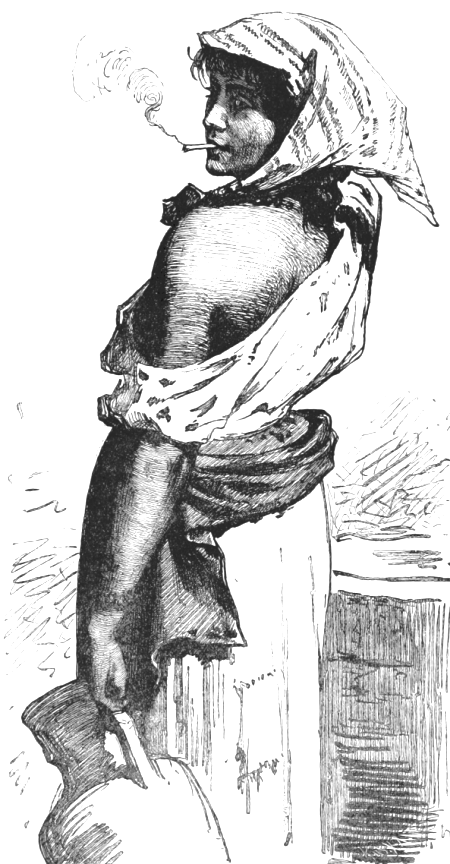
\includegraphics[scale=.5]{Charmer}
  \end{center}


  \cbreak


  \mysubsection{Aphrodite’s Sigh}{charm-aphrodites-sigh}

  By means of this spell you can create a ghostly moaning sound that appears to come from somehere Nearby. The moan is not loud nor can it quite cause fear, but any that hear it will know of it's "unnatural" nature. 

  \mysubsection{Candlelight}{charm-candlelight}

  This spell creates a small mote of light roughly equal to candle light that hovers near your head. The spell is typically used for reading or lighting a small area (half a cubic meter). This charm cannot be cast into someone's eyes. The light is dim enough that it's not particularly useful for lighting dark passages unless that passage is very well known (such as the your own home). 

  \mysubsection{Creature Comforts}{charm-creature-comforts}

  You can raise or lower the temperature of any non-living material a few degrees, enough to warm or cool food or drinks or a room.  The temperature cannot be raised to a degree where it would injure anyone.


  \mysubsection{Dowsing}{charm-dowsing}

  Using a forked wand of hazelwood, you can sense the direction of a substantial body of potable water.  It ignores "insignificant" amounts of water, as found in a waterskin or barrel.  The spell doesn’t tell you how hard it might be to get to the water.

  \mysubsection{Fastening}{charm-fastening}

  This spell allows you to close one door or window that is not locked or otherwise barred. This will not lock the door or window unless by the action of closing it naturally becomes locked. 

  \mysubsection{Flame of Vesta}{charm-flame-of-vesta}

  You may change a fire into one of black flame, so that it casts no light but still provides heat.  You can affect a normal fire up to the size of a campfire.  Furthermore, the flames do not burn, though they are uncomfortable to the touch.

  \mysubsection{Jinx}{charm-jinx}

  You can perform a minor hex by tracing a five pointed star in the air with your forefinger. The hex can affect something Nearby or closer.  These hexes can be severing a rope, shattering a pane of glass, spoiling a piece of food, or some other small act of malice.  Note that these hexes will not work if there is a Pooka nearby

  \mysubsection{Levitate}{charm-levitate}

  You may use this spell to lift an object via magic alone. The object needs to be non-living and weigh less than 1kg. The object will remain floating in mid-air for up to 1 Hour as long as you are paying at least some attention to it. If you are distracted at all, say in Combat or casting another spell (including another Charm) then the object drops. 

  \mysubsection{Matchstick}{charm-matchstick}

  When you drag your forefinger along a rough surface and says the name of Buer, your fingertip combusts like a giant phosphorus match. It burns for a Moment and does not hurt you in any way.

  \mysubsection{Message}{charm-message}

  By means of this spell you can send a brief message, no more than a dozen words, to a person you know. This person can be any distance away, but they have to be able to understand the language of the message you're sending.

  \mysubsection{Puff of Air}{charm-puff-of-air}

  This spell creates a small puff of air; enough to blow away dust from objects or to put out a candle, but not enough to put out a torch or lantern. The puff can move very light items as would a puff of air blown from natural means. This spell can be used to blow dirt from an item or area 1m by 1m. 

  \mysubsection{Spice}{charm-spice}

  This minor spell flavors one serving of food. The flavor can be changed but it does not change the nature of the food item nor does make poisoned food or spoiled food edible, similar to Freshen. The flavor can be chosen by you. 

  \mysubsection{Sweet Dreams}{charm-sweet-dreams}
  This spell allows you to make a willing creature fall asleep. The spell will not work if used against an unwilling subject. You can cast this spell on yourself, but this will be the last spell that you cast that day.

  If used on a subject who is already asleep, you can breathe in their ear and control what dreams they have the following night. No matter how unpleasant the dreams, this cannot prevent the victim from getting a full night’s rest on its own, but it can affect their mood.

  \mysubsection{Third Eye}{charm-third-eye}

  By holding or touching an inanimate object and concentrating for Minutes, you can detect whether or not something is magical in nature, or if something can "hold" an enchantment (including staves, swords, and holy relics).  

  Alternately, you can use this charm to "see" any Nearby concealed objects, like secret doors and hidden compartments.  The Charm doesn't detect invisible or magically concealed objects. 


  \mysubsection{Tidy}{charm-tidy}

  This spell can be used to clean a single object. The object can be anything, clothing, armor, weapons or even a area of a home. Unlike other Charms this one can be cast on a willing living participant. A warlock casting clean on themselves will appear as they would if they had recently bathed and donned fresh clothing. This spell can clean 1 cubic meter of space or an area 3m x 3m. 

  Alternately, you can fix minor wear and tear in non-living and non-metal apparel, fixing small rips and tears as if you were using a needle and thread.  The amount of material mended cannot exceed 1 cubic meter.  You cannot fix a dented piece of armor or sharpen a sword, but you could fix a pane of glass if all the pieces are present, or reattach a broken strap of a backpack

  Finally, you can use this charm to "freshen" one object up to 1 cubic meter. Typical uses are to remove the wrinkles in a garment, brighten the color or some non-living object, or even make bland food more favorable, or polishing metal or glass. All these effects are considered to be a minor illusion. This spell cannot make poisoned or spoiled food edible. 

  \mysubsection{Turkish Delight}{charm-turkish-delight}

  You can create a single piece of food or drink, such as a Turkish delight, a piece of fruit, or glass of wine. It is exquisitely delicious and provides no nourishment whatsoever. If not eaten within Minutes, it dissolves into black smoke.  If you have a Toxin, you can use it on this food.

  \cbreak

  \mysubsection{Unbolting}{charm-unbolting}

  This spell creates allows you to open one door, window, chest or other item that is not locked or otherwise barred. 

  \mysubsection{Watchdog}{charm-watchdog}

  You can place an area of alarm around themselves.  Any creature larger than a cat that comes Close or Nearby to you sets off a mental alarm that will wake you up from non-magical sleep.  You will not know what has entered the circle, but you will know something has, and the the general direction.


%%%%%%%%%%%%%%%%%%%%%%%%%%%%%%%%%%%%%%%%%%%%
%%% LEECHCRAFT
%%%%%%%%%%%%%%%%%%%%%%%%%%%%%%%%%%%%%%%%%%%%

    \newpage

    \mysection{Leechcraft}{arcana-leechcraft}


  \example {
    \mybold{Knowledge Die} + Modifiers vs. Target
  }

    Knowledge Dice are used in the pratice of \mylink{Leechcraft}{arcana-leechcraft}.   In order to perform the healing arts, you must roll your Knowledge Die vs. the Target (below).  Unless otherwise noted, Leechcraft requires 2 Actions to perform.  The recipient of the Leechcraft \mybold{cannot move} while you are applying your healing arts.   

    Your \INT can add a bonus to your roll:

    \mytable{X X}{
      \thead{\INT} & \thead{Bonus} \\
    }{
      d2-d10 & +0  \\
      d12 & +1  \\
      d16 & +2  \\
      d20 & +3  \\
      d24 & +4 \\
    }

   
  When applying Leechcraft, if you roll less than the Target number, your next roll is at -2.  This is cumulative:  -2 for the first miss, -4 for the second, etc.  These negatives are removed when you take a Bivouac.  When rolling, your \SUMDICE can never be less than 1.


  \LEECHCRAFT[
    Name=Bonesetting,
    Link=leechcraft-bonesetting,
    Target=9,
    Keywords=Purge,
    Reversible=Y
  ]

  Can only be performed during a Bivouac.  Purge a single non-serious Physical Wound.  If desired, you can use this 'craft to cause a non-serious Physical wound (your choice).  

  \LEECHCRAFT[
    Name=Delay Infection,
    Link=leechcraft-delay-infection,
    Target=7,
    Keywords=None,
    Reversible=Y 
  ]
  
  Can only be performed during a Breather or Bivouac.  Delay the onset of a single Disease (including contagion) for the rest of the Session.  If desired, you can use this 'craft to speed the disease along (Arbiter's discretion - the disease should move 1 "step" in a worse direction).

  Curing Disease requires \mylink{Medicinals}{research-medicinals}

  \begin{center}
  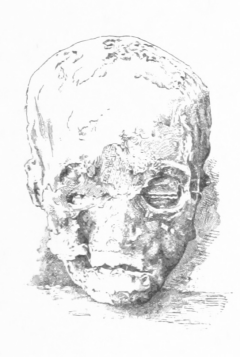
\includegraphics[scale=.5]{Skull}
  \end{center}


  \LEECHCRAFT[
    Name=Hair of the Dog,
    Link=leechcraft-hair-of-the-dog,
    Target=2,
    Keywords=Purge,
    Reversible=N
  ]

  Purge the effect of a Hang Over on a single person.

  \LEECHCRAFT[
    Name=Laudanum,
    Link=leechcraft-laudanum,
    Target=9,
    Keywords=Purge,
    Reversible=Y 
  ]

  Remove a Disgusted, Shaken, or Sickened effect on a single patient.  If applied during a Bivouac, Purge a single non-serious Mental Wound.   If desired, you can use this 'craft to cause a non-serious Mental wound (your choice) during a Bivouac.

  \LEECHCRAFT[
    Name=Mend,
    Link=leechcraft-mend,
    Target=2,
    Keywords=None,
    Reversible=Y
  ]

  Can only be applied to a patient who is Dying. Heal 1 Flesh.  

  You can also use Mend to cause a point of damage to a dying person (prompting a \DEATH roll).  The attempt isn't noticable to others unless they're practiced in Leechcraft.

  \LEECHCRAFT[
    Name=Purge Toxin,
    Link=leechcraft-purge-toxin,
    Target=6,
    Keywords=None,
    Reversible=N 
  ]

  Immediately purge a Toxin from the body of a single patient

  \LEECHCRAFT[
    Name=Restore Senses,
    Link=leechcraft-restore-senses,
    Target=6,
    Keywords=None,
    Reversible=N 
  ]
  Remove a Blindness or Deafness effect on a single patient

  \LEECHCRAFT[
    Name=Sew Wounds,
    Link=leechcraft-sew-wounds,
    Target=4,
    Keywords=None,
    Reversible=N
  ]
  You can only perform this during a Breather or Bivouac. The patient rolls 1 \FLESH and heals that much Flesh.

  \LEECHCRAFT[
    Name=Smelling Salts,
    Link=leechcraft-smelling-salts,
    Target=3,
    Keywords=Purge,
    Reversible=N
  ]
  Purge a Knocked Out effect on a single patient


  \LEECHCRAFT[
    Name=Staunch,
    Link=leechcraft-staunch,
    Target=4,
    Keywords=Purge,
    Reversible=Y
  ]
  Purge or cause a Bleed effect on a single patient


  \LEECHCRAFT[
    Name=Trepanation,
    Link=leechcraft-trepanation,
    Target=8,
    Keywords=Purge,
    Reversible=Y  
  ]
  You can only drill holes in peoples' heads during a Bivouac.  Purge a Woozy effect on a single patient.   If desired, you can use this 'craft to cause the patient to become Woozy instead.

  \LEECHCRAFT[
    Name=Virtigo,
    Link=leechcraft-virtigo,
    Target=6,
    Keywords=None,
    Reversible=Y 
  ]
  
  Bivouac only.  Purge a Befuddled or Concussed effect on a single patient.   If desired, you can use this 'craft to cause the patient to become Befuddled or Concussed


\newpage

%%%%%%%%%%%%%%%%%%%%%%%%%%%%%%%%%%%%%%%%%%%%
%%% Mysteries
%%%%%%%%%%%%%%%%%%%%%%%%%%%%%%%%%%%%%%%%%%%%

\mysection{Mysteries}{arcana-mysteries}


\mysubsection{Civilized}{arcana-mystery-civilized}
\MYSTERY [
  Name = Armor of the Gods,
  Link = arcana-mystery-armor-of-the-gods,
  Paradigm = Force,
  Save = N,
  Duration = Session,
  Target = Self
]

You cannot wear any other armor while you're wearing Armor of the Gods.  What the armor looks like is up to you, but it should be elaborate/brutal/gilded etc. - something that makes you stand out in a crowd.  Your \MD drops to d4; the \UD for the Armor depends on the number of \DICE invested: 1 d4; 2-3 d6; 4-6 d8; 7-9 d10; 10+ d12.

\MYSTERY [
  Name = Clamp,
  Link = arcana-mystery-clamp,
  Paradigm = Force,
  Save = Y (neg.),
  Duration = varies,
  Target = Nearby Target(s)
]

A clamp of red light appears over \DICE Monsters or objects you designate. The maximum width of the clamp is \DICE meters, and the clamp must be able to fit around the objects (so you wouldn't be able to clamp something to a floor or a wall).  The clamp will push the objects together until they are held securely, but it will not damage either object.  For example, you could clamp an orc to a chair or a sword to a table.  If one of the things clamped is a living thing, the creature can break free if they \RB : \VIG with a -\DICE penalty; otherwise, the duration depends on the number of dice spent:  1 [die]: Minutes; 2 \DICE: Days; 3 \DICE: Weeks; 4 \DICE: Months; 5 \DICE: Years; 6+ \DICE: Permanent.  Save negates.


\MYSTERY [
  Name = Divvy,
  Link = arcana-mystery-divvy,
  Paradigm = Entropy,
  Save = N,
  Duration = Permanent,
  Target = Close Target(s)
]

You can command something that's a mixture of different types (soup, coins, etc.) weighing no more than \DICE X50kg to separate into \DICE+1 categories.  The categories have to be clear and easily identifiable by inspecting them, and they have to be able to flow freely.  For example, you could split a soup into "vegetables" "broth" and "poison", or a pile of coins into "minted during the last century" and "older". You could not, however, split a pile of coins into "handled by Xerphion the Tyrant" and "not handled by Xerphion the Tyrant", as there's no way to tell just by inspecting them. You could not separate "a locked chest" and "its contents", because the items could not flow freely into separate piles.


\MYSTERY [
  Name = Exchequer,
  Link = arcana-mystery-exchequer,
  Paradigm = Entropy,
  Save = N,
  Duration = Instant,
  Target = Close Target(s)
]

You can convert up to \SUMDICE kg of coins into coins of another type of equivalent value (as a reminder, there are 100 coins in a kg, and 4kg of coins are 1 Significant Item). For example, if the \SUMDICE of your dice roll was 10 you could convert 1,000 iron pieces (10kg) into 100 silver pieces (1kg) or 10 gold pieces (1/10kg); or you could convert 10 gold pieces into 100 silver pieces or 1,000 iron pieces. Additionally, you can place up to \DICE X100kg of coins into "hammerspace" for an indefinite period of time; the coins essentially cease to exist, have no Burden, and cannot be stolen or taken by others (though the existence of the coins can be divined through a Scry spell or similar).  You can retrieve the coins at any time (though you have to retrieve all of them at once).  The coins are also released upon your death, meaning that you might occassionally be a target of thieves.
You can combine the effects above (so you could convert money and store it in hammerspace if you'd like).  You must cast this spell each time you want to put more coins into hammerspace, but everything that's in hammerspace is released upon your death.

  \begin{center}
  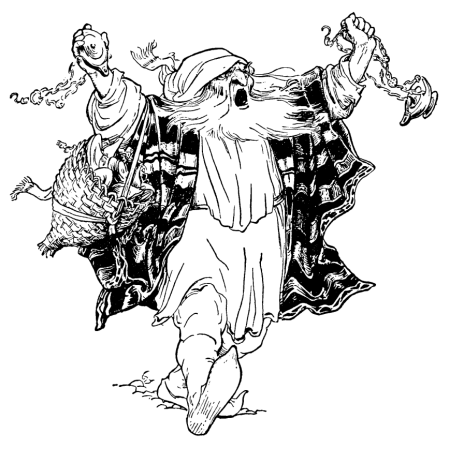
\includegraphics[scale=.5]{CivilizedArcana}
  \end{center}



\MYSTERY [
  Name = Forgehammer,
  Link = arcana-mystery-forgehammer,
  Paradigm = Force,
  Save = N,
  Duration = Session,
  Target = Self
]

A magical blacksmith's hammer appears in your hand that only you can wield.  The hammer deals \DICE damage up to a maximum of 8. You fight with this weapon using your \FOC (instead of your \VIG).  Every time the hammer deals damage, its damage goes down by 1.   Additionally, you can also repair the Max \UD of an Ally's armor during a Bivouac; for every \DCUP you repair in this way, the damage of the hammer goes down by 1.  Once the Forgehammer hits 0 damage, it disappears. The Forgehammer can strike creatures who are only struck by magical weapons, but because there is no die to roll when dealing damage, it cannot Crit or be Fumbled.

Once the damage die is exhausted (reaches 0), the Forgehammer disappears.


\MYSTERY [
  Name = Hone,
  Link = arcana-mystery-hone,
  Paradigm = Force,
  Save = N,
  Duration = Combat or \SUM Minutes,
  Target = Close Target(s)
]

You run your hands over \DICE metal, stone, or wooden edges and hone them to a razor sharpness. If the object is a Bashing weapon, it deals +\DICE damage; if the object is a Stabbing or Chopping weapon, it deals +\DICE X2 damage. The edge must be smaller than your outstretched arms.

\MYSTERY [
  Name = Millworks,
  Link = arcana-mystery-millworks,
  Paradigm = Entropy,
  Save = N,
  Duration = Instant,
  Target = Close Target(s)
]

A tree no larger than \DICE X 5m tall and \DICE meters in diameter topples over, as if neatly cut. The result depends on the dice you invest. 1 \DICE: cut and broadly de-limbed, 2 \DICE: cut, de-limbed, debarked, 3 \DICE: cut, de-limbed, debarked, cut into planks as per your specifications, stacked, 4 \DICE cut, planed, de-limbed, debarked, cut into planks, stacked, sanded, and finished. Small limbs and offcuts will be piled for kindling. Alternatively, you can reduce the tree to sawdust or wood chips in 20-\SUMDICE minutes


\MYSTERY [
  Name = Package Neatly,
  Link = arcana-mystery-package-neatly,
  Paradigm = Entropy,
  Save = n/a,
  Duration = Concentration or Permanent,
  Target = Nearby Target(s)
]

Up to \DICE X250kg of nonliving objects, as you designate, are packed neatly. You must name the objects or their general category when you cast the spell ("those coins", "the contents of that room") If no packing materials are provided, the objects will be stacked into compact cubes, with the largest and most stable objects at the bottom. If chests, paper and twine, sacks, carts, etc. are provided, the spell will use them as you direct. The packages created will take up the minimum space possible, and will be remarkably sturdy. The spell will continue to pack objects for as long as you maintain concentration. The objects must be able to move freely. You could not use this spells to pack clothes someone was wearing. The objects will not lift more than 3m off the ground during the packing process.

\mysubsection{Cthonic}{arcana-mystery-cthonic}
\MYSTERY [
  Name = Abyssal Trident,
  Link = arcana-mystery-abyssal-trident,
  Paradigm = Force,
  Save = N,
  Duration = Session,
  Target = Self
]

A magical trident appears in your hand that only you can wield.  The trident is a 2-handed weapon that deals \DICE+\DICE damage up to a maximum of 12.   You fight with this weapon using your \FOC (instead of your \VIG).  Every time the trident deals damage, its damage goes down by 1. The trident can strike creatures who are only struck by magical weapons, but because there is no die to roll when dealing damage, it cannot Crit or be Fumbled. 

Once the damage die is exhausted (reaches 0), the Abyssal Trident disappears.

\MYSTERY [
  Name = Davy Jones's Locker,
  Link = arcana-mystery-davy-joness-locker,
  Paradigm = Prophesy,
  Save = N,
  Duration = Instant,
  Target = Close Target(s)
]

You must be near a body of water to use this liturgy (a river is OK, a puddle isn't).  You summon a lock up to \DICE meters in length, width, and height.  The box can hold up to \DICE X100kg in weight, or about 25 Significant Items (provided the box is big enough in terms of height, width, and depth i.e. you could put a 2 meter long pole in a 1 [die] locker).  Once you seal the box and carve your name onto it, the waters will take the locker back beneath the surface, where it will disappear.  At any time, you can return to the same body of water and bring the locker back from the depths. Nothing else can bring the locker back from the deeps (not even the liturgy of Dredge) except your death.  When you die, the locker will wash up on shore within a few days for some lucky (or unlucky) soul to find.
If you place a living thing inside, it can breathe - but it will starve or die of thirst without food or water (incidentally, this is a great way to make \myital{vodyanoi})

\MYSTERY [
  Name = Dredge,
  Link = arcana-mystery-dredge,
  Paradigm = Mind,
  Save = N,
  Duration = Concentration,
  Target = Close or Nearby
]

Choose an area \DICE meters in radius.  Buried or covered objects rise \DICE x5 meters to the surface.  If you cast this spell on the ground, coins, stones, and roots will be pulled to the surface; if you cast it on water, sunken objects will rise to the surface and remain as long as you concentrate.  The objects cannot weigh more than \DICE x100kg.  

\MYSTERY [
  Name = Excavate,
  Link = arcana-mystery-excavate,
  Paradigm = Elements,
  Save = N,
  Duration = Instant,
  Target = Close
]

You can remove up to \DICE inorganic materials from a \DICE x5 meter cube just in front of your feet.  The materials could be "stone", "water", "dirt", etc. The materials disappear permanently. Objects that would be suspended in the material removed will obey the laws of physics - removing water will cause the surrounding water to rush in, removing dirt from around a chest will cause the chest to fall, etc.

\MYSTERY [
  Name = Fade,
  Link = arcana-mystery-fade,
  Paradigm = Mind,
  Save = Y (neg.),
  Duration = Markovian,
  Target = Nearby Target(s)
]

You can cause a Ally, Monster, or object to fade out of existence.  You can still see them, though they're insubstantial (like a ghost).  The target can't move, talk, or interact with the world in any way.  Not even magic can affect the target.  If the target is unwilling, it gets a Save to negate.  The duration is Markovian and depends on the number of \DICE invested.

  \begin{center}
  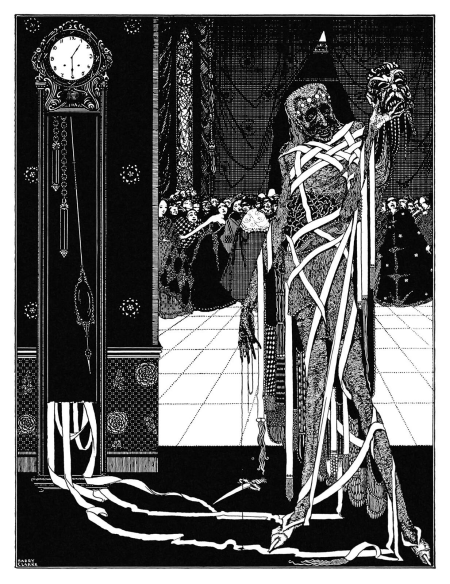
\includegraphics[scale=.5]{CthonicArcana}
  \end{center}


\MYSTERY [
  Name = Mermaid's Breath,
  Link = arcana-mystery-mermaids-breath,
  Paradigm = Biomancy,
  Save = Y (neg.),
  Duration = \SUM Minutes,
  Target = Self or Close Target(s)
]

For \SUMDICE Minutes, up to \DICE+1 Allies or Monsters (including yourself) can breathe water as if it were air.  They can only breathe water, however - breathing air will cause them to drown. Unwilling creatures get a Save to negate.  You must touch the Creature to bestow this mystery upon them. 

\MYSTERY [
  Name = Sinister Stillness,
  Link = arcana-mystery-sinister-stillness,
  Paradigm = Mind,
  Save = N,
  Duration = Combat or \SUM Minutes,
  Target = Close\, Nearby\, Far-Away\, or Distant
]

You can invoke this liturgy in an area  Close, Nearby, Far-Away, or Distant from yourself.  The air Close to the area takes on an unsettling air of silence.  Sound is not magically suppressed, but Monsters and creatures within its bounds feel that any sound they make will disturb something better left undisturbed.  Non-intelligent animals will not enter the area, and Monsters inside must make an immediate morale check. Thereafter, Saves against fear effects have a -\DICE penalty (minimum 1), and morale rolls suffer a -\DICE penalty.  A morale check is needed to enter or pass through the area of the spell.

\MYSTERY [
  Name = Sound the Deeps,
  Link = arcana-mystery-sound-the-deeps,
  Paradigm = Force,
  Save = N,
  Duration = Instant,
  Target = Close Target(s)
]

You slap your hand on the ground or the surface of the water.  The echoes of the tremor allow you to precisely know how deep and the approximate shape of bodies of water, chasms, shafts, clefts, mountain peaks, caverns, passages, etc.  up to a distance of [dice]x100m meters.  Additionally, you may use this to rouse up to \DICE Allies Close, Nearby, Far Away, or Distant who are Sleeping, Knocked Out, etc. 

\newpage

\mysubsection{Cunning}{arcana-mystery-cunning}
\MYSTERY [
  Name = Expertise,
  Link = arcana-mystery-expertise,
  Paradigm = Mind,
  Save = N,
  Duration = \SUM Minutes,
  Target = Self
]

Name a Skill - it can be one of the 7 basic skills, or any other skill you choose (though you can't learn things that would not be contained in a well stocked library, or that are so rare that only a few people could teach them to you).  You are Trained (d8) in that Skill for the spell's duration.  If you already know the Skill, add +\DICE x2 to your Skill roll.

\MYSTERY [
  Name = Illusion,
  Link = arcana-mystery-illusion,
  Paradigm = Mind,
  Save = N,
  Duration = Varies,
  Target = See Below
]

You create an illusion of anything you desire. If anything touches the illusion, it will pass through it with no effect.  The illusion cannot be greater than \DICE x \DICE meters in size.  Think of the illusion as a perfectly accurate hologram that you are creating - the illusion can be heard in addition to being seen, can perform the same action over and over again, and can deliver messages, but it can't interact in a meaningful way or perform complex actions based on external forces. 

Each aspect of the illusion requires one or more Faith to cast:

\mybullet {
  \item You want the illusion to say up to \DICE + \DICE words or make \DICE + \DICE sounds (wailing, shouting, etc)
  \item You want the illusion to be a physical thing (hole in the ground, stone wall, orc guard, etc)
  \item You want the illusion to be able to move up to \DICE meters
  \item You want to cast the illusion on a living creature (disguise them as a beggar or a lamp post)
}

Note that there is some Arbiter's discretion here.  A guard pacing in front of a door might cost 2 \DICE (a physical thing moving back and forth 2
meters), but if you want the illusion of acrobats or pouncing lions it will be more costly.  A disguise cast on someone to appear to be a beggar might
cost 1 [die] (a living creature wearing the face and clothing of a random beggar), but disguising yourself as the king will be significantly harder.

The Illusion will last for \DICE Hours.  Anyone touching the illusion will immediately know it to be fake, but this doesn't cause the illusion to
disappear.  However, if the illusion is touched with an \mylink{Ego Weapon}{wizardry-ego-weapon}, it will immediately disappear.

\MYSTERY [
  Name = Labyrinth,
  Link = arcana-mystery-labyrinth,
  Paradigm = Mind,
  Save = N,
  Duration = Combat or \SUM Minutes,
  Target = Self
]

You create a spiraling labyrinth of thought in your mind.  Anyone targeting you with Charm, Sleep, or any magical effect whereby the caster tries to read your mind or alter your memories must enter into a \RB : \FOC contest with you at a -\DICE penalty.  If they fail, they will be caught in your mind for the duration of the spell;  they immediately catch the Vapors, and you can hear all their thoughts.

  \begin{center}
  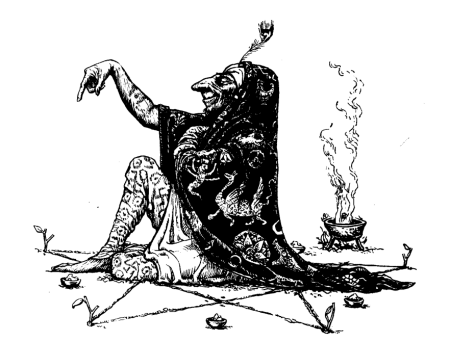
\includegraphics[scale=.5]{CunningArcana}
  \end{center}



\MYSTERY [
  Name = Memory Lane,
  Link = arcana-mystery-memory-lane,
  Paradigm = Mind,
  Save = Y (neg.),
  Duration = Varies,
  Target = Close Target(s)
]

You can create a memory (real or not) and embed it in the head(s) of up to \DICE creatures by touch.  Unwilling creatures may Save to negate the spell.  The memory must be short and distinct.  The memory will start to fade in a few days, but if you win a \RB : \FOC attempt against the victim (the victim has a -\DICE penalty) when you invoke the mystery, the memory will never fade, even if they lose all other memories (incidentally, this is is a really great way to create a ghost or poltergeist).

\MYSTERY [
  Name = Mirror Image,
  Link = arcana-mystery-mirror-image,
  Paradigm = Mind,
  Save = n/a,
  Duration = Minutes,
  Target = Self
]

You create \DICE illusory images of yourself, which move as you move and always stay Close to you. They are constantly stepping through each other, so that it is impossible to tell which is which. When an enemy attacks you, roll to see if they hit you or an image (equal chance). An image vanishes as soon as it suffers a solid impact (a blow from a mace, but also a slap). Area effects such as a dragon's breath will cause all images to instantly vanish (and you'll take fire breath damage, naturally).

\MYSTERY [
  Name = Paralysis,
  Link = arcana-mystery-paralysis,
  Paradigm = Mind,
  Save = Y (neg.),
  Duration = Markovian,
  Target = Close or Nearby Target(s)
]

Up to \DICE creatures of \DICE \HD or less must Save or be Paralyzed.  Sleeping creatures do not get a Save. The duration is Markovian and depends on the number of \DICE invested

\MYSTERY [
  Name = Strange Copy,
  Link = arcana-mystery-strange-copy,
  Paradigm = Mind,
  Save = N,
  Duration = \SUM Hours,
  Target = Close Target(s)
]

You reach into a mirror-like surface and pull out a copy of an object reflected in the mirror. The object that you pull out must be within reach of the mirror (as if it were a window), small enough to fit through the mirror (as if it were a window) and can't weigh more than \DICE x10kg. The mirror object looks and feels exactly like the object it copied, though it is a mirror image (so if you were to copy a book, the text would be backwards).  You can't copy any magical properties of the object, and you can only duplicate objects, not living things.  The object exists for \SUMDICE Hours.  If the object suffers a solid blow, it pops like a bubble.

\MYSTERY [
  Name = Twin,
  Link = arcana-mystery-twin,
  Paradigm = Mind,
  Save = N,
  Duration = \SUM Minutes,
  Target = Close Target(s)
]

You reach into a mirror-like surface and pull out a copy of yourself.  The mirrored surface has to be big enough for you to walk through - same height and same width, at least.  The copy behaves just like you, but it's illusory - anything that touches it will pass right through it, and it can't pick anything up or hold anything.  You can switch places with your mirror-self by stepping through the mirror - this dispels the illusion, and you appear wherever your mirror self is at the moment you step through.

\newpage

\mysubsection{Empyrean}{arcana-mystery-empyrean}
\MYSTERY [
  Name = Children of Shul,
  Link = arcana-mystery-children-of-shul,
  Paradigm = Prophesy,
  Save = Y (half),
  Duration = Session,
  Target = Self
]

You create \DICE small moons that circle the top of your head, casting moonlight Close and Nearby.  The shadows thrown by this moonlight give a +\DICE bonus to all Whispers made by Allies who are Close to you.  The moonlight will also activate abilities and powers that manifest in lunar rays (like lycanthropy), and throw light equivalent to \DICE candles.

You can unerringly throw one these moons at Nearby Monsters every Moment, striking for 3 damage each (including creatures only struck by Magic weapons).  When you have no moons left, the spell ends.

The moons can be dispelled at any time, but can only be summoned once a Session.

\MYSTERY [
  Name = Glorious Sunburst,
  Link = arcana-mystery-glorious-sunburst,
  Paradigm = Elements,
  Save = Y (half),
  Duration = Combat or \SUM Minutes,
  Target = See Below
]

You raise your hands to the heavens and fire a flare up to 50m upwards, where it hovers providing bright sunlight to all areas Close, Nearby, and Far-Away.  You can command the sunburst to change color, move horizontally, or explode.  No shadows can be cast beneath the sunlight (meaning sneaking around is difficult if not impossible), and all invisible creatures and objects appear with a thin halo around them the color of the sun.  Anyone who performs the sacrament Curse the Unhallowed while under the Glorious Sunburst adds an additional +\DICE to their damage; anyone Close to the sunburst if it explodes takes \SUMDICE+\DICE damage, Save for half.

\MYSTERY [
  Name = Lightning,
  Link = arcana-mystery-lightning,
  Paradigm = Elements,
  Save = Y (half),
  Duration = Instant,
  Target = Close or Nearby Target(s)
]

Forks of lightning erupt from your forehead, striking a Close or Nearby target for \SUMDICE+\DICE damage (Save for half). You can cause the lightning to "jump" up to \DICE-1 times to another creature or object Close by, provided they are conductive (iron armor, metal ladders, etc).  Magic swords aren't conductive.  You can "ping-pong" between two objects if you desire. Creatures struck by this secondary lightning bolt take \DICE damage (no Save). Objects struck by this secondary lightning bolt will become momentarily electrified, and deal a shock that could cause someone to lose their grip unless they \RO : \VIG + \FOC with a -\DICE penalty.

\MYSTERY [
  Name = Lunacy,
  Link = arcana-mystery-lunacy,
  Paradigm = Mind,
  Save = Y (neg.),
  Duration = Markovian,
  Target = Close or Nearby Target(s)
]

You invoke the madness of the moon.  \DICE creatures must immediately make a Sanity roll; if they do not have Sanity (Monsters, for instance) the creatures are permitted a Save.

The Lunacy is random for each Monster that fails its Save.  Roll a d4:  1) the Monster becomes Enraged; 2) the Monster becomes Afraid; 3) the Monster is Knocked Out; 4) the Monster suffers Anathema.  The duration is Markovian and depends on the number of \DICE used.

  \begin{center}
  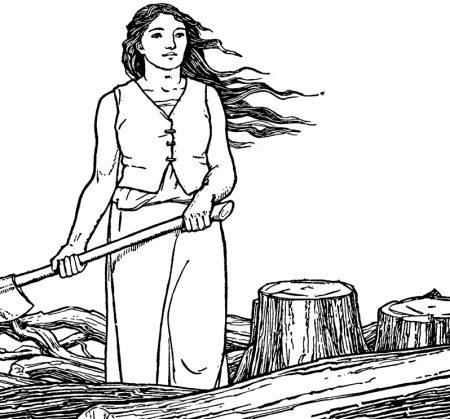
\includegraphics[scale=.5]{EmpyreanArcana}
  \end{center}


\MYSTERY [
  Name = Mountainhands,
  Link = arcana-mystery-mountainhands,
  Paradigm = Biomancy,
  Save = N,
  Duration = Session,
  Target = Self
]

Your hands enlarge and become stone.  Unarmed Attacks do an extra point of damage for every 2 \DICE you spend; in addition, you can reach your hands into substances that might affect Flesh but not stone (fire, boiling water - OK.  Lava or acid - not OK).  Holding a stone in your hands allows you to speak to it as the Murk ability (see the Core Rules). 

Your hands must be empty (including rings and gloves) in order to invoke this mystery. You can only invoke this mystery once per Session.

\MYSTERY [
  Name = Rainburst,
  Link = arcana-mystery-rainburst,
  Paradigm = Elements,
  Save = n/a,
  Duration = Combat or \SUM Minutes,
  Target = See Below
]

You create a rainstorm in the surrounding area.  The rain extinguishes all fires (even magical ones) for the duration, prevents non-magical fires from starting, and heals Allies and Monsters alike for \SUMDICE Flesh (once at the moment of invocation).  The range is dependent on the number of \DICE invested: 1 Close; 2-3 Close and Nearby; 4-6 Close, Nearby, and Far-Away; 7+ Close, Nearby, Far-Away, and Distant.

\MYSTERY [
  Name = Resonating Command,
  Link = arcana-mystery-resonating-command,
  Paradigm = Mind,
  Save = Y (neg.),
  Duration = Markovian,
  Target = Nearby Target(s)
]

You shout a one word command at up to \DICE Close or Nearby target, who must obey (Save negates).  The target(s) must be able to understand your language.  The command resonates for a Markovian duration - if the Markovian die is not a 1 or a 2, they must Save again.  Each Moment after the first the target(s) gain an additional +1 to their Save.  The command cannot directly cause the target(s) harm or force them to commit a harmful action.  You could cause them to run into a trap they didn't know was there, or into a tactically disadvantageous position, but not off a cliff.

\MYSTERY [
  Name = Thunderclap,
  Link = arcana-mystery-thunderclap,
  Paradigm = Elements,
  Save = Y (neg.),
  Duration = Instant,
  Target = Far-Away or Distant
]

You can invoke this mystery somewhere Far-Away or Distant from yourself.  Monsters Close to the Thunderclap must immediately make a morale check with a -\DICE penalty, or become Afraid.  Additionally, Monsters become Deafened for \DICE Moments unless they make a Save with a -\DICE penalty.

\newpage

\mysubsection{Errant}{arcana-mystery-errant}
\MYSTERY [
  Name = Armor of Winds,
  Link = arcana-mystery-armor-of-winds,
  Paradigm = Entropy,
  Save = n/a,
  Duration = Session,
  Target = Self
]

Take \DICE Faith and put them "in reserve".  For the remainder of the Session, you may sacrifice one of these [die] to cause any single \mybold{physical} attack that would damage you to miss instead of hit.  You must sacrifice the [die] \myital{before} you roll your Guard or Save.  You can only use 1 [die] per Moment.  Any unused \DICE are lost at the end of the Session.  You can only invoke this mystery once per Session.

\MYSTERY [
  Name = Capture Wind,
  Link = arcana-mystery-capture-wind,
  Paradigm = Elements,
  Save = N,
  Duration = Concentration or Session,
  Target = See Below
]

A magical circle \DICE meters in radius extends from your fingertip in front of you. As long as you maintain concentration, you can absorb any wind passing through the circle. You can then collapse the spell. 

At any time during the Session, you can reactivate the circle to release the wind you absorbed.  The wind flows out at the same rate it entered. If you activate this spell in a light breeze for 5 minutes, the spell will release a light breeze over 5 minutes. The wind only flows from the circle, so anyone standing behind it is not affected (unless you release hurricane-force winds indoors). You can cancel the release at any time, which expends the spell as usual. If you go to 0 Flesh while the spell is still "reserved", it immediately activates facing a random direction.  

If the wind is a magical breath that would do damage (dragon's breath, etc.) your \SUMDICE must be equal to or greater than the sum of the damage, or the circle immediately collapses.  

\MYSTERY [
  Name = Corsair's Blade,
  Link = arcana-mystery-corsairs-blade,
  Paradigm = Force,
  Save = n/a,
  Duration = Session,
  Target = Self
]

A magical rapier appears in your hand that only you can wield.  The rapier deals \DICE damage up to a maximum of 6.  You must make a successful Fight check using your \FOC (instead of \VIG or \DEX).  The Hero's Rapier ignores Armor and Soak, and while you wield it you always win Init.  Every time the rapier deals damage, its damage goes down by 1. The rapier can strike creatures who are only struck by magical weapons, but because there is no die to roll when dealing damage, it cannot Crit or be Fumbled.  

Once the damage die is exhausted (reaches 0), the Hero's Rapier disappears.


  \begin{center}
  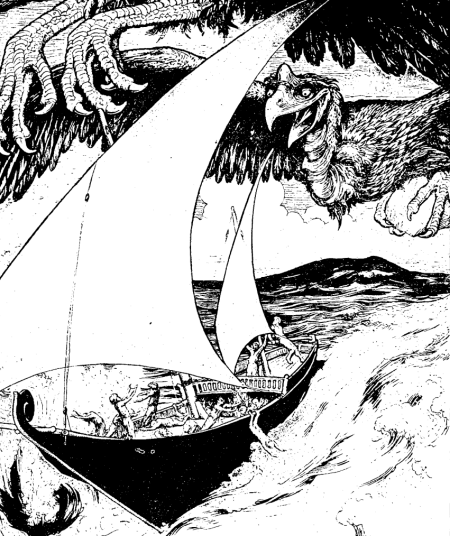
\includegraphics[scale=.5]{ErrantArcana}
  \end{center}



\MYSTERY [
  Name = Duelists' Wings,
  Link = arcana-mystery-duelists-wings,
  Paradigm = Biomancy,
  Save = n/a,
  Duration = Combat or \SUM Minutes,
  Target = Self or Close Target(s)
]

Tiny white wings sprout from the ankles and wrists of up to \DICE Allies.  They always win Init in Combat, and any falling damage is reduced by -\DICE per die.

\MYSTERY [
  Name = Ropework,
  Link = arcana-mystery-ropework,
  Paradigm = Entropy,
  Save = N,
  Duration = \SUM Minutes,
  Target = Close Target(s)
]

You summon a rope \DICE x50m in length.  You can command the rope to arrange itself into any shape and rise into the air in any orientation.  It can be climbed like a normal rope, and can support \DICE x100kg of weight.  Its ends do not need to be anchored to anything.

\MYSTERY [
  Name = Shatter Bonds,
  Link = arcana-mystery-shatter-bonds,
  Paradigm = Force,
  Save = n/a,
  Duration = Instant,
  Target = Close or Nearby
]

By invoking this mystery, you can sunder up to \DICE bonds either Close or Nearby.  The bonds may be physical (shackles, chains, or locks) or mental (Charm, Command, Labyrinth, etc) at the Arbiter's discretion.

\MYSTERY [
  Name = Skald's Tongue,
  Link = arcana-mystery-skalds-tongue,
  Paradigm = Entropy,
  Save = n/a,
  Duration = Breather or Bivouac,
  Target = Close Target(s)
]

This mystery can only be invoked during a Breather or Bivouac.  You play a rousing song, recite part of an epic, or sing an ancient ballad.  You can heal up to \SUMDICE+\DICE Grit among all Allies who listen, divvied up any way you want.

\MYSTERY [
  Name = Vaulting Step,
  Link = arcana-mystery-vaulting-step,
  Paradigm = Force,
  Save = N,
  Duration = Instant,
  Target = Self
]

Your next \DICE+\DICE strides (about 1m each stride) land on a plane of Force the size of your foot.  The step can be taken in any direction up, down, sideways, or across (though you cannot pass through physical objects).  You can combine these in any way you want - stride 45 degrees into the air, take another step up, and a final step down (for example).  Your final step must be on a solid surface, or you fall. 


\mysubsection{Heathen}{arcana-mystery-heathen}
\MYSTERY [
  Name = Barkskin,
  Link = arcana-mystery-barkskin,
  Paradigm = Biomancy,
  Save = Y (neg.),
  Duration = Combat or \SUM Minutes,
  Target = Self or Close Target(s)
]

You or a creature you target is covered in heavy bark.  Weight is increased by \DICE x100kg and all physical damage is reduced by -\DICE for the duration of the spell, but you can't swim, jump, or run. If invoked on something already in deep water, mud, etc. the target will immediately sink at x\DICE the normal rate. Unwilling creatures get a Save to negate. 

\MYSTERY [
  Name = Bloodvine,
  Link = arcana-mystery-bloodvine,
  Paradigm = Biomancy,
  Save = N,
  Duration = Instant,
  Target = Close or Nearby Target(s)
]

This spell can only be used on a Monster who suffering from the Bleeding effect.  Vines erupt from the Monster's wounds, dealing \SUMDICE+\DICE damage (no Save).  If the damage kills the Monster, their corpse is entirely consumed in a bramble of vines

\MYSTERY [
  Name = Butterfly Hurricane,
  Link = arcana-mystery-butterfly-hurricane,
  Paradigm = Biomancy,
  Save = Y (neg.),
  Duration = Combat or \SUM Minutes,
  Target = Self
]

A whirling brightly colored mass of butterflies springs into being around you, cloaking you and anyone else Close to you.  Any ranged attacks fired into or out of the hurricane automatically miss (AoE effects like dragon's fire aren't affected).  Anyone inside of the hurricane must Save or become Befuddled for as long as they remain inside - you and up to \DICE Allies are immune.

\MYSTERY [
  Name = Clearwater,
  Link = arcana-mystery-clearwater,
  Paradigm = Elements,
  Save = n/a,
  Duration = Instant,
  Target = Self or Close Target(s)
]

This mystery can only be invoked during a Breather or a Bivouac.  You create \DICE draughts of cold, clear water that have one of the following effects:

\mynumlist {
    \item Restore \DICE Flesh
    \item Restore \SUMDICE Grit
    \item Immediately end the effect of a Toxin
    \item Immediately end the effect of a Disease
}

\MYSTERY [
  Name = Elemental Spray,
  Link = arcana-mystery-elemental-spray,
  Paradigm = Elements,
  Save = Y (half),
  Duration = Instant,
  Target = Close or Nearby Target(s)
]

You emit \DICE sprays of elements from your fingertips that you can split among \DICE Monsters.  For each Monster, if the \SUMDICE of the \DICE targeting the Monster is greater than the Monster's \HD, they take \DICE+\DICE fire damage.  If the \SUMDICE is twice the Monster's \HD or more, they also take \DICE+\DICE cold damage.  If the \SUMDICE is three times the Monster's \HD or more, they also take \DICE+\DICE lightning damage.  If the \SUMDICE is four times the Monster's \HD or more, they also take \DICE+\DICE acid damage.  Save for half.

\MYSTERY [
  Name = Entangling Smoke ,
  Link = arcana-mystery-entangling-smoke,
  Paradigm = Elements,
  Save = Y (neg.),
  Duration = Markovian,
  Target = Close or Nearby Target(s)
]

This spell requires the Narcotic: Pipeweed.  You breathe out a plume of smoke; up to \DICE creatures or objects are grabbed by tendrils of this smoke unless they Save.  Those who fail move at half speed (meaning it takes 2 Maneuvers to move somewhere Nearby; for Monsters, it means their speed is Slow if it isn't already).  Any Ally fighting this Monster gains a +\DICE bonus to Fight and Guard. The duration is Markovian and depends on the number of \DICE invested.

\MYSTERY [
  Name = Hearthfire,
  Link = arcana-mystery-hearthfire,
  Paradigm = Elements,
  Save = n/a,
  Duration = Bivouac,
  Target = Close Target(s)
]

During a Bivouac, you may perform up to \DICE effects, once per die (though you may choose an effect multiple times):
\mybullet {
\item Repair the \MAX \UD of an Allies armor to full
\item Provide Provisions for 1 Ally
\item Heal up to \DICE Flesh on 1 Ally
\item Prevent any Wandering Monasters from attacking your camp
}

  \begin{center}
  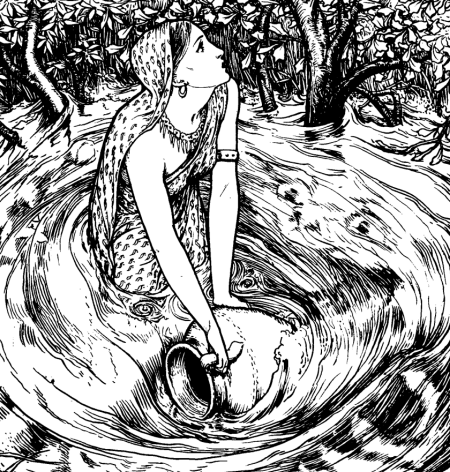
\includegraphics[scale=.5]{HeathenArcana}
  \end{center}



\MYSTERY [
  Name = Sporous Breath,
  Link = arcana-mystery-sporous-breath,
  Paradigm = Biomancy,
  Save = Y (neg.),
  Duration = Combat or \SUM Minutes,
  Target = Nearby Target(s)
]

You breathe a cloud of mushroom spores into an area Nearby.  All Allies and Monsters are affected by the Sporous Breath unless they make their Save.  The effects depend on the number of \DICE used: 1-3 all targets suffer Anathema; 4-6 all targets are Woozy; 7-9 all targets are Befuddled; 10+ all targets are affected with an Iron (d4) Toxin.

Only yourself and Pooka are immune to the effects of the Sporous Breath.

\mysubsection{Jötnar}{arcana-mystery-jötnar}
\MYSTERY [
  Name = Dirge,
  Link = arcana-mystery-dirge,
  Paradigm = Death,
  Save = n/a,
  Duration = Concentration,
  Target = Close Target(s)
]

You begin droning a hero's dirge.  For as long as you concentrate, all Close and Nearby Allies gain a +\DICE bonus to their \DEATH checks.

\MYSTERY [
  Name = Extinguish,
  Link = arcana-mystery-extinguish,
  Paradigm = Elements,
  Save = N,
  Duration = Instant,
  Target = Close or Nearby Target(s)
]

Beams of slushy ice shoot from your outstretched hands and strike up to \DICE targets.  If the target is on fire, the flame is immediately extinguished.  Flames the size of torches only require 1 [die]; people or animals would require 2 \DICE; bonfires and the like require 3+ \DICE at the Arbiter's discretion.

\MYSTERY [
  Name = Giantform,
  Link = arcana-mystery-giantform,
  Paradigm = Biomancy,
  Save = n/a,
  Duration = Combat or \SUM Minutes,
  Target = Self
]

You grow \DICE x 500cm in height, with strength to match.  Your Unarmed Attacks do an extra point of damage for every 2 \DICE you spend, and you can lift an additional \DICE x100kg.   If you are wearing Armor when you invoke Giantform, you take \MAX \UD in Flesh damage, and the Armor is ruined (drops to 0 \MAX \UD).  You are unable to use "normal" sized weapons while in Giantform.

\MYSTERY [
  Name = Incinerate,
  Link = arcana-mystery-incinerate,
  Paradigm = Elements,
  Save = N,
  Duration = See Below,
  Target = Close Target(s)
]

This mystery requires you to create a bonfire.  You can place up to \DICE inorganic objects into the fire weighing no more than \SUMDICE kg.  The objects are burned to a pile of enchanted ash, which can be harvested and stored as an Insignificant item.  When you wish the objects to become whole again, you must build a fire and sprinkle the ash inside of it; you can reach into the fire unharmed to pull the objects from the flames as they were when you placed them into the fire.  If you perish before the objects are retrieved, the ash reverts to normal, unenchanted ash and the objects are destroyed.


  \begin{center}
  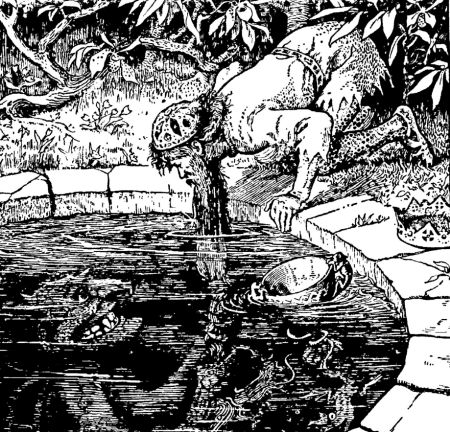
\includegraphics[scale=.5]{JotnarArcana}
  \end{center}



\MYSTERY [
  Name = Preserve,
  Link = arcana-mystery-preserve,
  Paradigm = Elements,
  Save = Y (neg.),
  Duration = varies,
  Target = Close Target(s)
]

By touching an object, you are able to freeze it for a period of time in order to preserve it.  If the object is an Ally or Monster, they must be lying completely still in order to use the liturgy.  Unwilling creatures get a Save.  While frozen, any toxins, diseases, bleeding, or negative effects are stopped for a period of time, depending on the number of dice spent.  You cannot end this liturgy willingly once it has begun, though it could be ended prematurely by great heat (a very large bonfire, for example) or by taking more than \SUMDICE points of damage, which will cause the object to shatter into many pieces.  

1 [die]: Minutes; 3 \DICE: Days; 5 \DICE: Weeks; 7 \DICE: Months; 9 \DICE: Years; 11+ \DICE: Permanent. 

\MYSTERY [
  Name = Ray of Fire,
  Link = arcana-mystery-ray-of-fire,
  Paradigm = Elements,
  Save = Y (neg.),
  Duration = Instant,
  Target = Nearby or Far-Away Target(s)
]

A narrow beam of fire shoots from your outstretched finger.  Make a Fight roll using your \FOC+\DICE; if you hit, the target catches fire for a Markovian duration if they fail a Save.  They are only allowed 1 Save.  They damage taken by the target is whatever is rolled on the Markovian die each Moment.  The beam of fire will also light flammable things alight.

\MYSTERY [
  Name = Trollblood,
  Link = arcana-mystery-trollblood,
  Paradigm = Death,
  Save = n/a,
  Duration = Combat,
  Target = Self
]

This mystery can be invoked at any time during Combat.  As long as you are alive, you regenerate +\DICE Flesh at the bottom of each Moment.  This regeneration is negated if the damage is from an acid or fire source. At the end of Combat, this mystery immediately ends (before you can take a Breather).

\MYSTERY [
  Name = Witness Me,
  Link = arcana-mystery-witness-me,
  Paradigm = Death,
  Save = n/a,
  Duration = Combat,
  Target = Self
]

This mystery can only be invoked in Combat.  For the remainder of Combat, you gain +\DICE on your Fight checks, and deal +\SUMDICE damage when you hit (rolled each time along with your damage).  At the end of Combat, you immediately catch the Vapors and drop to 0 Flesh, and must make a \DEATH check.

\newpage

\mysubsection{Monstrous}{arcana-mystery-monstrous}
\MYSTERY [
  Name = Dragonbreath,
  Link = arcana-mystery-dragonbreath,
  Paradigm = Elements,
  Save = Y (half),
  Duration = Instant,
  Target = Nearby
]

You breathe out a gout of dragon's breath before you.  The breath deals \SUMDICE+\DICE damage to all creatures Nearby, Save for half damage (plus see below).  The type of breath is random, roll a d6 for the type of breath: 1) Fire (Red); 2) Acid (Black); 3) Frost (White); 4) Lightning (Blue); 5) Corrosive Gas (Green); 6) Void (Bone).  The additional effect of the dragon's breath is as follows:

\mybullet {
  \item \mybold{Red:}   Fire.  If you fail your Save, you catch fire.  Take d4 damage at the top of each Moment until you spend an entire Moment doing "stop, drop, and roll".  This can be shortened to a single Maneuver if someone helps you.
  \item \mybold{Black:}  Acid.  If you fail your Save, take d4 acid damage for d4 Moments
  \item \mybold{White:}  Frost.  If you fail your Save, you are knocked Prone
  \item \mybold{Blue:}  Lightning.  If you fail your Save \mybold{and} are wearing metal armor, take an additional 1 point of damage per die
  \item \mybold{Green:}  Corrosive gas.  If you fail your Save, reduce your Soak by 1, or roll your  Armor \UD
  \item \mybold{Bone:}  Void.  If you fail your Save, you catch the Vapors for d4 Markovian
}

\MYSTERY [
  Name = Harpy's Talons,
  Link = arcana-mystery-harpys-talons,
  Paradigm = Force,
  Save = n/a,
  Duration = Session,
  Target = Self
]

Your fingers sprout iron-hard talons.  The talons can strike for \DICE damage each up to a maximum of 4.  You can strike with both of these Talons in Combat at the same time; roll your Fight die twice using your \FOC (instead of your \VIG).  If both talons hit, the Monster is also afflicted with Bleeding.  Every time your talons deal damage, their damage goes down by 1 (you tell the Arbiter which Talon goes down in damage, either "left" or "right"); when \mybold{one} of the Harpy's Talons hits 0 damage, the talon disappears (you can still strike with the other talon, but it won't have the Bleeding effect). The talons can strike creatures who are only struck by magical weapons, but because there is no die to roll when dealing damage, it cannot Crit or be Fumbled

\MYSTERY [
  Name = Serpent's Fang,
  Link = arcana-mystery-serpents-fang,
  Paradigm = Biomancy,
  Save = n/a,
  Duration = Combat or \SUM Minutes,
  Target = Self
]

Make your Fight \RO using your \FOC.  If you succeed, you grapple a Monster and may immediately bite them with your fangs.  The Monster takes \DICE damage and begins Bleeding, unless they Save.  You may apply Toxins to your fangs, but if you do so you must \RS : \FOC or accidentally ingest the Toxin, with the appropriate negative effects.

\MYSTERY [
  Name = Slimeform,
  Link = arcana-mystery-slimeform,
  Paradigm = Biomancy,
  Save = n/a,
  Duration = \SUM Minutes,
  Target = Self
]

You transform yourself and all of your Gear into a slime.  You can absorb up to \SUMDICE+\DICE damage without any ill effects (damage after this goes straight to Flesh, and immediately ends the mystery).  You are unable to attack, talk, cast spells, etc while in Slimeform, but you can move at a the pace of a slow walk, climb walls, hang from the ceiling, and slip under the cracks of doors if you wish.

\MYSTERY [
  Name = Spidertongue,
  Link = arcana-mystery-spidertongue,
  Paradigm = Biomancy,
  Save = Y (neg.),
  Duration = Combat or \SUM Minutes,
  Target = Self
]

You can speak with spiders (and they can speak with you).  Small spiders know about water, wind, and bugs.  Larger spiders know about people (maybe they can tell them apart).  Big, dangerous spiders know all kinds of things.  Spiders will be friendly towards you, but if you attack them they'll fight back.  Additionally, your spittle becomes a Toxin whose power depends on the number of \DICE spent: 1 [die] Iron Toxin; 3 \DICE Silver Toxin; 6 \DICE Gold Toxin.  Your spittle is enough to poison a drink, a needle or syringe, or infect someone you might bite, but not enough to poison a knife or dagger.  The spittle becomes normal when the duration ends.


  \begin{center}
  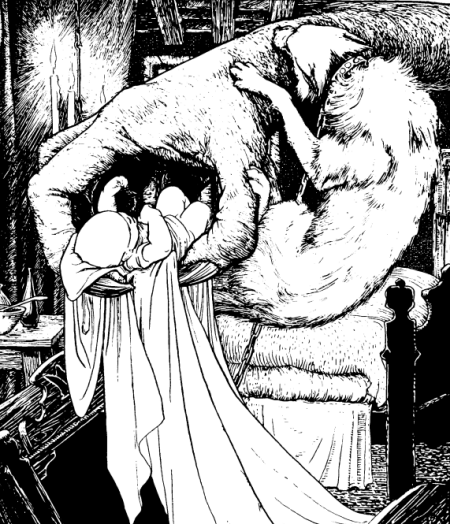
\includegraphics[scale=.5]{MonstrousArcana}
  \end{center}


\MYSTERY [
  Name = Tasty,
  Link = arcana-mystery-tasty,
  Paradigm = Biomancy,
  Save = N,
  Duration = Combat or \SUM Minutes,
  Target = Close Target(s)
]

The target object or Monster (alive or dead) smells delcious for the spell's duration.  The smell radiates Nearby in calm air, but can spread on the wind, or leave a trail.  Non-intelligent zoological creatures and swarms will be attracted to and attempt to eat the object or Monster first (even if they are supposed to be allies); intelligent creatures get a Save at a -\DICE penalty. 

\MYSTERY [
  Name = Tattered Robe,
  Link = arcana-mystery-tattered-robe,
  Paradigm = Entropy,
  Save = Y (neg.),
  Duration = Combat or \SUM Minutes,
  Target = Self
]

You must be wearing robes without armor to use this liturgy.  The edges of your robes form into \DICE tatters, each of which can be used as a weapon in combat in addition to your regular attack. The tatters deal no damage and each of their attacks must be rolled separately using your \FOC instead of your \VIG or \DEX - but if you hit the target begins Bleeding unless they make a Save.  You can split these attacks among as many Close opponents as you desire.

The tatters can also be used to hold small objects, as if they were each a prehensile tail.  Each tatter can hold up to 50kg of weight, but cannot attack if they are holding something.

\MYSTERY [
  Name = Undead Visage,
  Link = arcana-mystery-undead-visage,
  Paradigm = Death,
  Save = n/a,
  Duration = Combat or \SUM Minutes,
  Target = Self
]

You turn yourself into a hideous undead caricature of your "normal self".  You immediately become Unhallowed and gain the following effects, based on the number of \DICE spent:  1-2 you are immune to spells from the Mind Paradigm; 3-4 you are immune to Toxins; 5-6 you are immune to spells of the Force paradigm; 7+  you are immune to iron weapons.  These effects are cumulative.

You can only speak Graveborn for the duration of the spell.  Your Undead form prompts a Sanity or morale check among all who see you (Allies and Monsters alike), unless they have seen you in your Undead form before. 


\mysubsection{Righteous}{arcana-mystery-righteous}
\MYSTERY [
  Name = Crusader's Helm,
  Link = arcana-mystery-crusaders-helm,
  Paradigm = Force,
  Save = n/a,
  Duration = Session,
  Target = Self
]

You summon an ivory basinet, complete with crest, neck guard, and visor.  While worn, the Crusader's Helm protects you as a normal helmet (ignore certain Physical Wounds, etc), and you can absorb up to \DICE spells of the Mind paradigm without effect.  With the visor down you can detect Invisible creatures and are immune to Surprise (including the Drop).

\MYSTERY [
  Name = Grounding Mantra,
  Link = arcana-mystery-grounding-mantra,
  Paradigm = Elements,
  Save = Y (neg.),
  Duration = Markovian,
  Target = Close\, Nearby\, or Far-Away Target(s)
]

By invoking this liturgy, you shackle up to \DICE creatures to the ground.  They must be touching the ground already when you make the invocation.  The creatures must keep at least one limb touching the ground at all times.  If they attempt to run, they must \RB : \DEX with a -\DICE penalty.  If they are knocked Prone, they must \RB : \VIG with a -\DICE penalty to stand up.  Save negates.

\MYSTERY [
  Name = Holy Weapon,
  Link = arcana-mystery-holy-weapon,
  Paradigm = Force,
  Save = n/a,
  Duration = Session,
  Target = Self
]

A holy weapon (describe to the Arbiter) appears in your hands that only you can wield.  The weapon is a 2-handed weapon that deals \DICE damage up to a maximum of 10.  In addition, you deal +\DICE damage against Unhallowed creatures. You fight with this weapon using your \FOC (instead of your \VIG). Every time the weapon deals damage, its damage goes down by 1; when it hits 0, the weapon disappears.  The trident can strike creatures who are only struck by magical weapons, but because there is no die to roll when dealing damage, it cannot Crit or be Fumbled. 

\MYSTERY [
  Name = Purging Fire,
  Link = arcana-mystery-purging-fire,
  Paradigm = Elements,
  Save = N,
  Duration = \SUM Minutes,
  Target = See Below
]

This mystery requires you to create a bonfire.  Up to \DICE Allies can step into the flames of the Purging Flames; each Moment they remain inside of the fire; they take 2 damage to Flesh, but can activate 1 of the following effects:

\mynumlist {
    \item Immediately end a Markovian effect;
    \item Immediately remove a Curse;
    \item Immediately remove a non-serious Spiritual wound;
    \item Immediately purge a Toxin
}

Anyone inside of the Purging Flames cannot lie, and must answer truthfully any question asked of them


  \begin{center}
  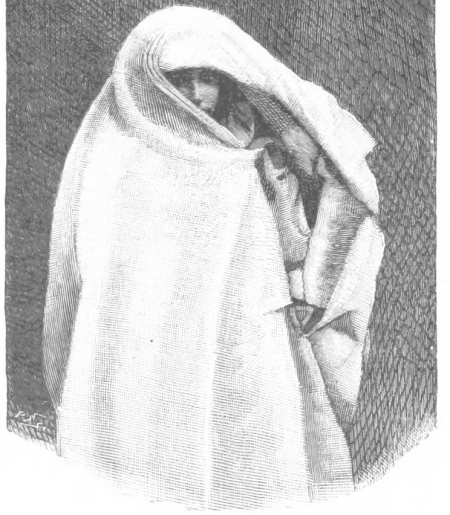
\includegraphics[scale=.5]{RighteousArcana}
  \end{center}



\MYSTERY [
  Name = Revered Aegis,
  Link = arcana-mystery-revered-aegis,
  Paradigm = Force,
  Save = n/a,
  Duration = Session,
  Target = Self
]

Take \DICE Faith and put them "in reserve".  You summon a brightly mirrored shield that can be Splintered (see the Combat Actions under Core Rules) up to \DICE times before it disappears.  Note that Splintering your shield is a Combat Action, and it ends your Moment; conversely, if you already took a Combat Action this Moment, you can’t Splinter your the Revered Aegis.  Any unused \DICE are lost at the end of the Session.  You can only invoke this mystery once per Session.

\MYSTERY [
  Name = Sacred Mail,
  Link = arcana-mystery-sacred-mail,
  Paradigm = Force,
  Save = n/a,
  Duration = Session,
  Target = Self
]

You can't wear any other armor while wearing Sacred Mail.  The mail appears as a glimmering suit of chainmail.  Your \MD drops to d8; the \UD for the Armor depends on the number of \DICE invested:  1-3 d4; 4-6 d6; 7-9 d8; 10+ d10.

\MYSTERY [
  Name = Satanic Verses,
  Link = arcana-mystery-satanic-verses,
  Paradigm = Entropy,
  Save = See Below,
  Duration = Instant,
  Target = Close
]

Books, scrolls, and parchment with writing on them burst into holy flame.  You can affect all writing in a \DICE meter radius around you.  If a Grimoire or Fetish is in possession of another (that is, on their person):
\mybullet {
\item the Grimoire will not catch fire if the Philosopher can \RB : INT vs. your \FOC.  They gain a bonus modifier for every spell in the Grimoire, but a -\DICE penalty on their roll.
\item the Fetish will not catch fire if the owner can \RB : \INT vs. your \FOC.  They may add the Fetish's \UD to their roll (and if they roll a 1 or a 2, the \UD moves \DCDOWN), but take a -\DICE penalty
}
If the Grimoire or Fetish is not in a persons' possession at the time the mystery is invoked, it does not get a Save.

Sigils will similarly catch aflame if they are unable to \RS using a d24.  Minor Sigils get a +2, Major Sigils get a +4, and Primary Sigils get a +8.  

The mystery has no effect on Tatoos or spells written in the heads of Philosophers.  This mystery is indiscriminate in what writing it will set alight.


\MYSTERY [
  Name = Sonorous Seeker,
  Link = arcana-mystery-sonorous-seeker,
  Paradigm = Prophesy,
  Save = N,
  Duration = \SUM Minutes,
  Target = See Below
]

You create a fluttering star of light that twitters like a bird.  Name an object using up to \DICE words - it can be a person ("the Stygian witch") or a thing ("the nearest body of water" or "the cask of Amontillado").  It has to be something you've seen clearly before.  Once named, the seeker will fly to it at the speed of an arrow and hover near it, chiming as loud as a bell.  If the object is not within the spell's range, it will try to find a similar object; otherwise, it disappears.


\mysubsection{Ruinous}{arcana-mystery-ruinous}
\MYSTERY [
  Name = Doombolt,
  Link = arcana-mystery-doombolt,
  Paradigm = Force,
  Save = Y (half),
  Duration = Instant,
  Target = Far-Away Target(s)
]

Target takes \SUMDICE+\DICE damage, Save for half. You do not need to see the target, but you do need to know their approximate location, and there must be a clear path a bolt could trace to reach them. The path can be as convoluted as required. The bolt can pass through gaps as small as a fist.  Note that this spell can only target Far-Away creatures.

  \begin{center}
  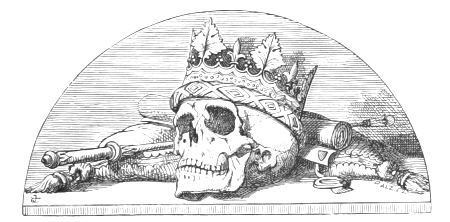
\includegraphics[scale=.5]{SkullLine}
  \end{center}



\MYSTERY [
  Name = Gaze of the Void,
  Link = arcana-mystery-gaze-of-the-void,
  Paradigm = Entropy,
  Save = Y (neg.),
  Duration = Instant,
  Target = Nearby or Far-Away Target(s)
]

A Monster disintegrates into nothingness. The number of \DICE invested must be twice the Monster's \HD + 1 (for example, to disintegrate a 1 \HD creature, you must invest 3 \DICE (1x2+1), a 2 \HD requires 5 \DICE, etc.) Monsters get a +2 to their Save; magical objects and magical monsters (dragons, unicorns, etc) get a +4 to their Save.



\MYSTERY [
  Name = Kismet,
  Link = arcana-mystery-kismet,
  Paradigm = Entropy,
  Save = n/a,
  Duration = Session,
  Target = See Below
]

Take \DICE Faith and put them "in reserve".  For the remainder of the Session, you may roll one of these [die] to modify \myital{any} \RO or \RB roll (by Ally or Monster alike) either plus or minus the \SUMDICE of the die roll.  You can only use 1 [die] per roll.  Regardless of the \SUMDICE of the [die], the Faith die is lost the moment it is rolled.  Any unused \DICE are lost at the end of the Session.  You can only invoke this mystery once per Session.

\MYSTERY [
  Name = Limbbreaker,
  Link = arcana-mystery-limbbreaker,
  Paradigm = Biomancy,
  Save = Y (neg.),
  Duration = Markovian,
  Target = Far-Away Target(s)
]

The target of this spell must have limbs.  With a snap of the fingers, \DICE of the target's limbs bend, crack, and break.  If an arm is broken, anything held in the hand is immediately dropped; if a leg is broken, the creature falls Prone; if both arms are broken, nothing can be picked up (and no spells can be cast); if both legs are broken, the Monster can only crawl.  The limbs remain broken for the Markovian duration, after which they immediately heal with no ill effects. Save negates.  Note that this spell can only target Far-Away creatures.

\MYSTERY [
  Name = Shrikeblast,
  Link = arcana-mystery-shrikeblast,
  Paradigm = Force,
  Save = Y (half),
  Duration = Instant,
  Target = Far-Away Target(s)
]

You let out a scream which shatters into shards of force.  The shards can lacerate up to \DICE  Far-Away Monsters and deal \SUMDICE+\DICE total damage (divided up any way you want).  If a Monster is killed by this spell, it will be suspended in the position it was killed for \SUMDICE Minutes by by the shards. A suspended creature is capable of bearing up to its own body weight in additional pressure before falling.  Note that this spell can only target Far-Away creatures.

\MYSTERY [
  Name = Storm of Hammers,
  Link = arcana-mystery-storm-of-hammers,
  Paradigm = Force,
  Save = Y (half),
  Duration = Concentration,
  Target = Far-Away Target(s)
]

Invisible hammers of Force strike up to \DICE Monsters from every direction.  Target Monsters take \DICE Bashing damage each, depending on how you split the die (Save for half).  The liturgy lasts for as long as you Concentrate.  Concentration and spell-casting is impossible while being struck by these hammers. Note that this spell can only target Far-Away creatures.

\MYSTERY [
  Name = Vermin Swarm,
  Link = arcana-mystery-vermin-swarm,
  Paradigm = Biomancy,
  Save = n/a,
  Duration = Concentration,
  Target = Close or Nearby
]

You summon a swarm of vermin that crawl up from the ground, walls, and ceiling.  The swarm can be directed for as long as you Concentrate and have a Base Speed (d16, 2 Maneuvers).  The swarm has \SUMDICE Health and deals \DICE damage to all Monsters Close to them provided a successful Fight roll is made (roll your \FOC for your Fight check).  Swarms take double damage from attacks that affect multiple targets, and share their Health equally as one "pool".  

\MYSTERY [
  Name = Wall of Gloom,
  Link = arcana-mystery-wall-of-gloom,
  Paradigm = Mind,
  Save = See Below,
  Duration = Markovian,
  Target = Nearby or Far-Away
]

You can anchor a barrier of pure darkness between three or more solid points up to \DICE meters in radius (for example: the 4 points of a door, two trees and the ground, across a hallway, etc).  Monsters that touch the blackness must immediately make a morale check with a -\DICE penalty or become Afraid for a Markovian duration.  Creatures that make their morale check that then continue through the wall must make a second Save; if they fail, they exit the wall the same way they came in (they will need to make a morale check again to touch the wall if they wish to try to move through it again).   






%%%%%%%%%%%%%%%%%%%%%%%%%%%%%%%%%%%%%%%%%%%%
%%%  NECROMANCY
%%%%%%%%%%%%%%%%%%%%%%%%%%%%%%%%%%%%%%%%%%%%
\newpage

\mysection{Necromancy}{arcana-necromancy}

To reach through the veil between life and death is to plunge your hands into the black rivers surrounding the Isle of the Dead.  Necromancy is abhorrent to Hallowed creatures; there are those who insist that Necromancy defies \TheAuthority, while others insist that it would not be possible if it were not permitted.  


Necromancy requires the \mylink{Crux of Mojo}{mortal-crux-mojo}, and is divided into three loose groups:  Black Magic, Carnomancy, and Corpse Witching.  Each Necromantic spell has a "Target" associated with it - you must this number or greater using your Mojo.  You can try as many times as you like, but if you roll a 1 or a 2, your Mojo moves \DCDOWN.  Rolling your Mojo in this way is a Maneuver Action.


\mysubsection{Black Magic}{arcana-necromancy-black-magic}

\NECRO[
  Name=Born of the Grave,
  Link=necromancy-born-of-the-grave,
  Paradigm=Death,
  Save=N,
  Duration=Session,
  Target=4
]

Requires a sniff of \mylink{Corpse Salt}{necromancy-corpse-salt}.  In addition to the Salt's narcotic abilities (see the Core Rules), you become as on born of the grave:

\mybullet {
    \item You take on a sickly/ghostly/rotting aspect.   You have \SUM additional Flesh while you are in this form.
    \item You are Unhallowed, breathe dirt as if it were air, have Darkvision, and can speak Graveborn fluently
    \item Any Allies that see you for the first time must roll their Sanity.  Monsters must roll their morale
    \item Shades and the Walking Dead will ignore you (unless you mess with them)
}

The effect can be ended at will; otherwise, it lasts until the end of the Session

\NECRO[
  Name=Crown of Thorns,
  Link=necromancy-crown-of-thorns,
  Paradigm=Death,
  Save=N,
  Duration=Session (see below),
  Target=5
]

A crown of blackberry thorns criss-crosses your forehead; blood leaks from your scalp.  Similar to the Virtue of Aura (see Core Rules), you use your Mojo as an Armor \UD in Combat.  Anyone who strikes you physically (including missile weapons) must Save or immediately take the Bleeding effect.  

The effect can be ended at will; otherwise, it lasts until the end of the Session or until your Mojo is exhausted.


  \begin{center}
  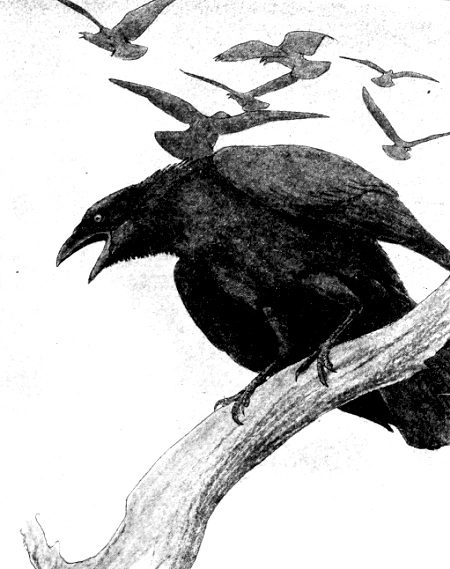
\includegraphics[scale=.5]{Crow}
  \end{center}


\NECRO[
  Name=Laughin' Jack,
  Link=necromancy-laughin-jack,
  Paradigm=Death,
  Save=N,
  Duration=0,
  Target=2
]

In a burst of blue flame and a whiff of brimstone, Laughin' Jack appears in your hand.  Jack appears as the blackened and burned skull of an infant, roughly the size of a grapefruit.  He emits a guttering, bluish corpselight from his eyes and mouth (treat as candlelight); if no one is looking at him, he whispers and chatters to himself in a language no one understands.  You may throw Jack (as a Throw weapon, obviously) using your \FOC instead of your \DEX.  Jack explodes for d4+1 damage on impact, and is able to strike creatures only hit by magic.  Throwing Jack counts as a Combat Action.



\NECRO[
  Name=Storm of Crows,
  Link=necromancy-storm-of-crows,
  Paradigm=Death,
  Save=Y (neg.),
  Duration=Concentration,
  Target=3
]

An inky murder of crows bursts from the ground in a whirling cloud, cloaking you and anyone Close to you.  For as long as you maintain Concentration, any ranged attacks fired into or out of the hurricane automatically miss (AoE effects like dragon's fire aren't affected).  

\mysubsection{Carnomancy}{arcana-necromancy-carnomancy}

\example{
    Using Carnomancy on an Ally requires them to make a \RS Sanity check. 
}


\NECRO[
  Name=Canopic Jar,
  Link=necromancy-canopic-jar,
  Paradigm=Death,
  Save=N,
  Duration=Session,
  Target=4
]

You can reach into your body and pull out yours or an Ally's stomach, intestines, lungs, or liver - and store them in Hammerspace.  You can only store 1 organ per personin Hammerspace at a time.  For each person after the first, the Target increases by +1 (for example, you could store your stomach in Hammerspace, the paladin's lungs [the Target would 5], and the wizard's stomach [the Target would be 6]).  While the organ is stored in Hammerspace, you (or your Ally) are Unhallowed.  Unwilling participants get a Save.

\mybullet {
    \item \mybold{Stomach:}   You do not need to eat or drink
    \item \mybold{Intestines:}  You can heal Grit even if an effect (like a specific wound) would normally prevent you from doing so
    \item \mybold{Lungs:}  You no longer need to breathe (this makes talking impossible)
    \item \mybold{Liver:}  You are not affected by any ingested Toxins.  If performed while under the effect of the Toxin, the Toxin is removed from the body (and placed in Hammerspace).  The Toxin must be dealt with when the liver is (presumably) returned to the body.
}

The Covenant of Blood allows you to do the following:

\NECRO[
  Name=Corpse Tongue,
  Link=necromancy-corpse-tongue,
  Paradigm=Death,
  Save=N,
  Duration=Session or \SUMDICE Minutes,
  Target=3
]

Using Corpse Tongue requires \mylink{Corpse Salt}{necromancy-corpse-salt}

\mybullet{ 
    \item \mybold{Corpse Smoke:} The Corpse Salt is mixed with pipeweed and Smoked (eliminating its Narcotic effects).  You gain the languages, memories, and Skills of the corpse for the rest of the Session (but not any spells, supernatural abilities, Virtues, etc.).  If the creatures particularly powerful (Arbiter's discretion), you must Save vs. hexes of gain some aspect of the creature's personality for the duration of the Session.  If the creature was over 100 years old, you must \RS : Sanity.  
    \item \mybold{Speak with Dead:}  You spread the Corpse Salt on a flat surface (be careful it doesn't blow away!)  The corpse will answer questions for \SUMDICE Minutes (the Arbiter will start a timer).  The dead only speak in Graveborn.  They will answer honestly, but the words tend to be cryptic and unhelpful, especially if the creature has no reason to help you.  Corpses usually don't remember exactly how they died.
}


\NECRO[
  Name=Covenant of Blood,
  Link=necromancy-blood-sacrament,
  Paradigm=Death,
  Save=Y (see below),
  Duration=see below,
  Target=2 (see below)
]

The Covenant of Blood allows you to do the following:

\mybullet {
    \item You can anoint someone with blood from your pricked finger.  They are Unhallowed until the end of the Session.  Unwilling creatures get a Save.
    \item Add +4 to the Target (6).  This rite can only be performed during a Bivouac.  You transfer blood from one creature to another; both creatures must be alive at the time of the transference.  Each Moment, the "donor" loses 1 point of Flesh, and the "recipient" gains 1 point of Flesh.  If the donor is brought to 0 Flesh during the transference, the recipient must Save vs Doom or fall to 0 Flesh, prompting a roll of their \DEATH
    \item Add +8 to the Target (10),  You heal from drinking another sentient creature's blood.  You may perform this liturgy during a Breather or Bivouac.  The creature must be alive when you feast on them; the act of drinking their blood takes their life.  Heal yourself to full Flesh and Grit.

}


  \begin{center}
  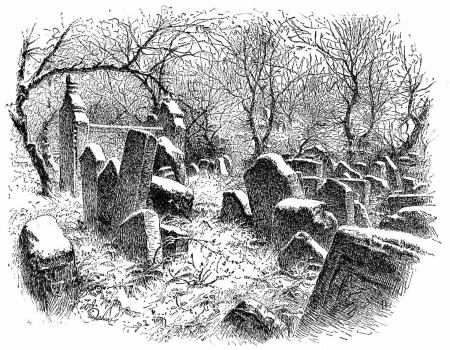
\includegraphics[scale=.5]{Graveyard}
  \end{center}


\NECRO[
  Name=Knit Flesh,
  Link=necromancy-knit-flesh,
  Paradigm=Death,
  Save=N,
  Duration=0 or Session,
  Target=2 (see below)
]

You heal 1 \HD of Flesh on a single creature. The healed flesh will appear grey and bloodless; wounds are sealed with wire and crude staples.  Horrible scars are usually left behind. You can only do this once per creature during a Breather or Bivouac (before you restore any Mojo).

You can also stitch a lost limb or hand to a stump.  Doing this increases your \mybold{Target} by +2 (4).   This requires an available limb of the appropriate size.  The limb rots quickly and a new one needs to be attached each Session.  The Witch also can "feel" what the limb feels (i.e. they can tell if the creature is holding something [but not what], if the creature is walking or running, etc).  While the stitched limb is attached, the creature is Unhallowed.


\mysubsection{Corpse Witching}{arcana-necromancy-corpse-witching}

\example{
    Corpse Witching must be performed on a corpse, no more than 7 days dead (by the law of \TheAuthority).  Corpse Witching consumes (destroys) the corpse
}


\NECRO[
  Name=Corpse Salt,
  Link=necromancy-corpse-salt,
  Paradigm=Death,
  Save=N,
  Duration=0,
  Target=2
]

You create d4 \UD of Corpse Salt, a coarse and gritty distillation that can be stored in a tiny pouch or vial.  Corpse Salt is a necessary component in certain Necromantic arts, and a Narcotic sought out by Philosophers (see Narcotics under the Core Rules).


\NECRO[
  Name=Death Scythe,
  Link=necromancy-death-scythe
  Paradigm=Death,
  Save=N,
  Duration=Session or Until Exhausted,
  Target=4
]


The corpse disintegrates as you pluck a black scythe from its center of mass. The scythe is 2 Handed and does d8 damage; this d8 is a \UD - when you exhaust the \UD, the scythe disappears.  Against Monsters of the same type, the scythe has the Weapon Trait: Cleave (for example, a scythe made from a troll corpse would have Cleave against trolls.) The scythe is only usable by you and counts as a magic weapon; it does not count as a Significant Item. You must make a successful Fight check using your \FOC (instead of \VIG or \DEX) to hit with the weapon.

\NECRO[
  Name=Exploding Corpse,
  Link=necromancy-exploding-corpse,
  Paradigm=Death,
  Save=N,
  Duration=Combat,
  Target=3
]

A corpse Close or Nearby to you explodes in a shower of bone and blood.  Anyone Close to the corpse must Save vs Hexes or take \SUMDICE damage.  Makes a really big fucking mess.



\NECRO[
  Name=Zombie,
  Link=necromancy-zombie,
  Paradigm=Death,
  Save=N,
  Duration=Session or Conc.,
  Target=5
]

\mybullet{
    \item \mybold{Slave:} You raise a corpse to help with mundane tasks, test for traps, etc.  The corpse moves very slowly (d3 \MD) but doesn't need to eat, sleep, rest, or breathe.  The corpse cannot Fight or Guard, and any damage to it (including Curse the Unhallowed) immediately destroys the Zombie.  The corpse has the strength of a normal person and can carry 25kg worth of stuff without tiring, but it'll need to be strapped to them (in a backpack or whatever).  Arbiter gets final say on what's allowed. The corpse can obey one word commands i.e. "dig", "sit", "go", "stop", etc.  The corpse can only understand Graveborn. It is completely mindless and extremely literal. The corpse will obey your last command until the spell's duration expires.  When the spell ends, the corpse falls to the ground and is immediately consumed.

    \item \mybold{Warrior:}  Creating a Warrior adds +3 to the Target (8).  The corpse is raised and will fight for you for as long as you maintain Concentration.  The Zombie uses your Mojo to Fight and Guard; you can raise as many Warriors as you wish, but they each use your Mojo to Fight and Guard. If you exhaust your Mojo or cease Concentration, the corpse falls to the ground and is immediately consumed.

}


\MONSTERBLOCK[
  Name=Zombie (Monster Stats),
  Link=necromancy-zombie-stats,
  MV=Slow*,
  WK=d20,
  DMG=2d4 1 Close,
  HD=2,
  Power=Strong,
  Soak=0,
  Morale=n/a,
  Save=2,
  Extras={Pack}
]

Zombies always go last in Combat. Zombies will try to grapple and bite automatically on following Moments. Zombie are Pack creatures (gain +1 damage for every Nearby zombie)




%%%%%%%%%%%%%%%%%%%%%%%%%%%%%%%%%%%%%%%%%%%%
%%%  SEVEN SACRAMENTS
%%%%%%%%%%%%%%%%%%%%%%%%%%%%%%%%%%%%%%%%%%%%

\newpage

    \mysection{Sacraments}{arcana-seven-sacraments}

    The Seven Sacraments are invoked by Mystics through the \mylink{Gift of Grace}{mystic-grace}


  \begin{center}
  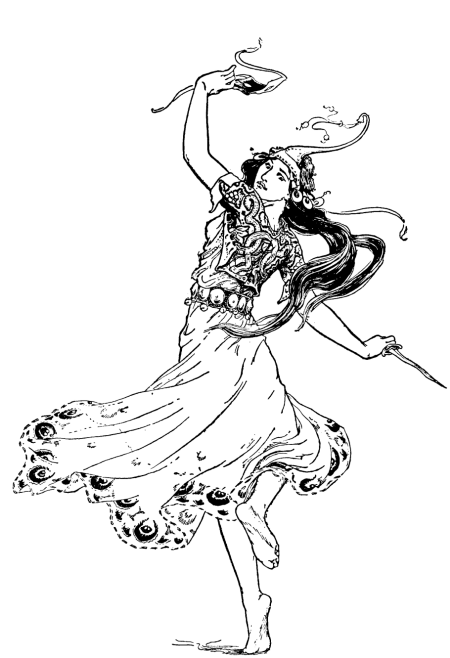
\includegraphics[scale=.5]{Sacraments}
  \end{center}


    \SACRAMENT [
      Name=Bless,
      Link=mystic-sacrament-bless,
      Paradigm=Grace,
      Save=N,
      Duration=Session,
      Counter=None,
      Keywords=Splittable,
      Target=Close Ally or object
    ]

    Choose one effect per Grace die invested: 
    1. The Ally can make a Save at a 6-in-6; 
    2. The Ally's can automatically succeed on a \RO or \RS check;
    3. The Ally can immediately end a Markovian duration affecting them;
    4. The Ally or object is Hallowed for the remainder of the Session (this negates the detriment Unhallowed)

    Once an effect is used, it disappears (though the Blessing can be recast)

    \SACRAMENT [
      Name=Consecrate,
      Link=mystic-sacrament-consecrate,
      Paradigm=Grace,
      Save=N,
      Duration=Concentration,
      Counter=None,
      Keywords=None,
      Target=Close radius
    ]

    You exude a \DICE meter diameter circle of \mylink{Hallowed Ground}{miracle-hallowed-ground} around yourself. You cannot move or be carried while concentrating on this Sacrament.

    Note that the area of Hallowed Ground will temporarily cancel out the effects of \mylink{Unhallowed Earth}{occultism-unhallowed-earth} (making it "normal"), but that Sacraments cannot be performed while you are on Unhallowed Earth.

   \SACRAMENT [
      Name=Curse the Unhallowed,
      Link=mystic-sacrament-curse-the-unhallowed,
      Paradigm=Grace,
      Save=Y,
      Duration=0,
      Counter=None,
      Keywords=Splittable,
      Target=\DICE Nearby Unhallowed
    ]


    Up to \DICE Unhallowed creatures take \SUMDICE + \DICE damage (Save for half).  You can divide this damage up any way you like.

    \example {
      Oberlan Xi, Mystic of Pilzesser, performs the sacrament of Curse the Unhallowed on a ghoul and a group of skeletons. He rolls 3 d4 Grace dice in the attempt and gets a 9 - adding the number of \DICE he rolled, this becomes a 12 (9+3).  He can affect up to 3 creatures, and decides to deal 6 damage to the ghoul and 3 damage to two of the skeletons (he could also have just dealt 12 damage to the ghoul if he preferred).
    }  


    \SACRAMENT [
      Name=Heal,
      Link=mystic-sacrament-lay-on-hands,
      Paradigm=Grace,
      Save=N,
      Duration=Concentration,
      Counter=None,
      Keywords=None,
      Target=Close (touch) Allies
    ]

    Heal up to \SUMDICE points of Flesh by touch. You may distribute healing among as many creatures as you would like, as long as the total Flesh healed does not exceed \SUMDICE and you maintain concentration. If you invest 4 \DICE or more, you may instead heal a single target's Flesh fully






   \SACRAMENT [
      Name=Loaves and Fishes,
      Link=mystic-sacrament-loaves-and-fishes,
      Paradigm=Grace,
      Save=N,
      Duration=0,
      Counter=None,
      Keywords=None,
      Target=Close radius
    ]


    You create enough food to feed \SUMDICE people for one meal, along with clean water to fill one mug per person. Mugs, utensils, and condiments are not provided.  Those that participate in the meal do not need to roll Provisions for a Bivouac.  

    \SACRAMENT [
      Name=Meditation,
      Link=mystic-sacrament-meditation,
      Paradigm=Grace,
      Save=N,
      Duration=0,
      Counter=None,
      Keywords=0,
      Target=Self
    ]

    You drop into deep meditation.  It needs to be quiet-ish, so you can't do it during Combat.  You can do up to \DICE of the following (you can only choose each option once per Meditation):
    \mylist {
        \item a) Heal 1 \UD of damage to an Intangible Stat
        \item b) Roll your \FOC and heal that much Flesh (up to \MAX)
        \item c) Roll your \FOC and heal that much Grit (up to \MAX)
        \item d) Purge yourself of a Toxin
    }


    \cbreak


    \SACRAMENT [
      Name=Walk on Water,
      Link=mystic-sacrament-walk-water,
      Paradigm=Grace,
      Save=N,
      Duration=Concentration,
      Counter=None,
      Keywords=Splittable,
      Target=Self and \DICE-1 Close (touch) Allies
    ]

    You and up to \DICE-1 Allies can slowly walk over water for as long as you maintain Concentration. 



%%%%%%%%%%%%%%%%%%%%%%%%%%%%%%%%%%%%%%%%%%%%
%%%  WIZARDRY
%%%%%%%%%%%%%%%%%%%%%%%%%%%%%%%%%%%%%%%%%%%%
  \newpage

  \mysection{Wizardry}{arcana-wizardry}

\SPELL[
  Name=Acid Arrow,
  Link=wizardry-acid-arrow,
  Paradigm=Elements,
  Save=N,
  Duration=0/Markovian,
  Counter=None,
  Keywords=None,
  Target=Nearby or Far-Away Monster or Object
]

You throw an acidic arrow at a Monster or object. You must make a successful Fight check using your \INT (instead of \VIG or \DEX).  If you succeed: 

\mynumlist {
  \item If the target is wearing Armor, they must make a \UD check at the start of every Moment for the Markovian duration of the spell.  If they are using a shield, they may immediately sunder it to nullify the spell; 
  \item If they are not wearing Armor, they must take \DICE additional damage at the start of every Moment for the Markovian duration of the spell; 
  \item If the target is an object, it will melt a \DICE x 10cm cubic area of wood, metal, or stone.  
}

\SPELL[
  Name=Arcadia's Bulwark,
  Link=wizardry-arcadias-bulwark,
  Paradigm=Mind,
  Save=N,
  Duration=Session,
  Counter=\mylink{Acid Arrow}{wizardry-acid-arrow},
  Keywords=None,
  Target=Self
]


A spectral shield with a heraldric device of your choosing appears in the vicinty of your non-dominant arm.  The shield moves on its own to block Throw and Shoot weapons, and can absorb up to \SUMDICE + \DICE damage before it dissipates.  You can also Sunder this shield (like the Combat ability),
which also causes it to dissipate. You can still cast spells while this shield is summoned.  An Acid Arrow fired into the shield will dispel it if a Wizards' Duel is lost.


\SPELL[
  Name=Balthazar's Breathtaking Blast,
  Link=wizardry-balthazars-breathtaking-blast,
  Paradigm=Biomancy,
  Save=Y (negate),
  Duration=Markovian,
  Counter=\mylink{Mighty Lungs}{wizardry-mighty-lungs} ,
  Keywords=None,
  Target=Nearby or Far-Away point
]

A marble-sized bead of poo lands at a Nearby or Far-Away point you select. You can cause the sphere to detonate at any time in \DICE Hours (including immediately). All creatures Close or Nearby the sphere's detonation must
Save or immediately become Sickened, and the area is filled with a thick green mist that lasts for \DICE Hours.  Any who enter the mist during this time must Save or become Sickened, though you smell it and see it before
you're in it, so you won't stumble into it blindly.  Animals will avoid the area for the Markovian duration.  The spell does not affect creatures with no sense of smell, mindless creatures, or creatures who habitually live in
filth (goblins, shambling mounds, etc.).  The mist can be dispelled by Mighty Lungs if a Wizards' Duel is lost.




\SPELL[
  Name=Bastogne's Glamping Charm,
  Link=wizardry-bastognes-glamping-charm,
  Paradigm=Force,
  Save=N,
  Duration=Bivouac,
  Counter=\mylink{Morass}{wizardry-morass} ,
  Keywords=None,
  Target=Close
]



In an area you designate, a magical camp appears where you and \DICE-1 allies can Bivouac. The camp includes a bedroll, a sleeping platform, a small purple and gold tent, a small table and chair, a kettle, a cookpot
with a stew going, an iron arm to hold the kettle or cookpot over a fire, a book entitled "The Erotic Poems of Plumtarch" (less erotic than expected), and a pair of dry wool socks for up to \DICE people. Any items removed from
the area vanish instantly. In the spell's area, the temperature is moderated very slightly, wind and rain are lessened, and vermin cannot enter.  The tents are immune to casual attack, including from wandering Monsters (anyone
sleeping outside the tents might not be so lucky).  Up to \DICE people staying at the camp can forego a single Provisions \UD roll during their Bivouac.  The campsite can be utterly dispelled by Morass if a Wizards' Duel
is lost.

\SPELL[
  Name=Battering Beam,
  Link=wizardry-battering-beam,
  Paradigm=Force,
  Save=N,
  Duration=Concentration,
  Counter=\mylink{Battering Beam}{wizardry-battering-beam},
  Keywords=Contested,
  Target=Close or Nearby Monster or Object
]


A beam of force erupts from your forehead and strikes something you can see, pushing it backwards. Every Moment, the creature or object is pushed 5m in the direction you are looking.  If it's an object, you can push up to \DICE
x100kg.  If it's a creature, they can make a Contested roll using \VIG with a -\DICE penalty to fight back. If you lose the Contest, the spell immediately ends - otherwise, the spell lasts as long as you concentrate. 
If the target cannot move backwards, it takes \DICE damage.  The Battering Beam can be dispelled by another Battering Beam if a Wizards' Duel is lost.




\SPELL[
  Name=Cacaphony,
  Link=wizardry-cacaphony,
  Paradigm=Entropy,
  Save=Y (negate),
  Duration=Varies,
  Counter=\mylink{Negasonic Bomb}{wizardry-negasonic-bomb} ,
  Keywords=None,
  Target=Nearby or Far-Away point
]



You roll a small orb of Entropy to a point Nearby or Far-Away; the orb rolls silently and is hard to see.  At any time for the next \SUMDICE Hours, you can have the orb detonate into an incredibly loud clattering, wailing, and
whistling. Creatures Close to the designated point must Save or be Stunned for \DICE Moments. It is audible in clear air up to a \DICE km away. You can designate \DICE conditions under which the orb will detonate. For example,
you could say "now"; "if anyone steps on it"; or "if water touches it".  The conditions must be obvious and must occur within 1m of the orb. When the spell's duration expires, you can choose to have the orb detonate (as above)
or vanish silently.  The Cacaphony can be dispelled by a Negasonic Bomb if a Wizards' Duel is lost.





\SPELL[
  Name=Charm,
  Link=wizardry-charm,
  Paradigm=Mind,
  Save=Y (negate),
  Duration=Session,
  Counter=\mylink{Charm}{wizardry-charm} ,
  Keywords=Contested,
  Target=Close Monster(s)
]



Ensorcel one or more Monsters whose combined \HD is less than or equal to \DICE.  Save negates; otherwise, they will regard you as a good friend and ignore the obvious spell you just cast on them.  The effect lasts for the
entire Session unless you ask them to do something they might think was a little weird: attack an ally, let you through an area they're supposed to be guarding, etc. (this is up to the Arbiter's discretion).  This prompts a
Contested roll by the victim, using \FOC with a -\DICE penalty.  You must touch the targets' flesh (like with a handshake) to cast the spell.  The charmed person must stay Close, Neary, or Far-Away from you - if you ever
move beyond this distance, the spell is ended.  The Charm can be broken and dispelled by another Charm if a Wizards' Duel is lost. 

  \begin{center}
  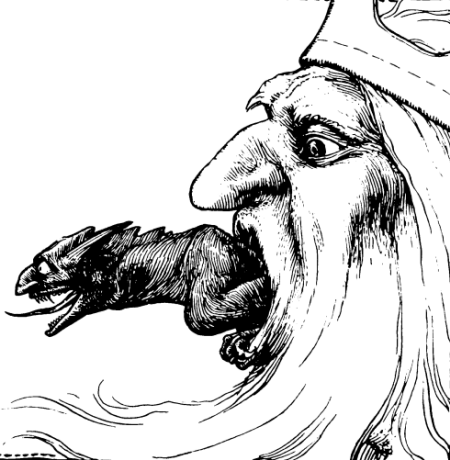
\includegraphics[scale=.5]{Tongue}
  \end{center}


\SPELL[
  Name=Color Spray,
  Link=wizardry-color-spray,
  Paradigm=Mind,
  Save=Y (negate),
  Duration=0 / Markovian,
  Counter=None ,
  Keywords=Splittable,
  Target=Close or Nearby Monster(s)
]



You emit \DICE sprays of color from your fingertips that you can split among \DICE Monsters.  For each Monster, if the \SUMDICE of the \DICE targeting the Monster is twice as much (equal to or greater) as the Monster's \HD, it
is Befuddled (the duration is Markovian and depends on the number of dice invested).  If \SUMDICE is three times the Monster's \HD, it is Stunned for a Moment, then Befuddled as above. If \SUMDICE is five times the creature's
\HD, it is Stunned (the duration is Markovian and depends on the number of dice invested), then Befuddled (Markovian duration).  Save negates.





\SPELL[
  Name=Commanding Presence,
  Link=wizardry-commanding-presence,
  Paradigm=Mind,
  Save=N,
  Duration=Combat or \SUMDICE Minutes,
  Counter=\mylink{Balthazar's Breathtaking Blast}{wizardry-balthazars-breathtaking-blast} ,
  Keywords=None,
  Target=Self
]

You grow +\DICE meters in height, and your features and voice become terrible and commanding.  Creatures of less than \DICE \HD must test morale or flee in terror.  You can use your \INT in place of any rolls where you
would normally use \VIG.  If you enter the radius of Balthazar's Breathtaking Blast, or if the spell is cast Close to you, the Commanding Presence is dispelled if a Wizards' Duel is lost.




\SPELL[
  Name=Ego Weapon,
  Link=wizardry-ego-weapon,
  Paradigm=Mind,
  Save=N,
  Duration=Session,
  Counter=\mylink{Greaseball}{wizardry-greaseball} ,
  Keywords=None,
  Target=Self
]



You can summon a Bashing, Cutting, or Stabbing weapon of Force.  You can change the type of weapon by using 1 Maneuver in Combat.  The weapon does \DICE damage and can hit creatures only affected by magic.  Only you can fight with the Ego Weapon.   You must make a successful
Fight check using your \INT (instead of \VIG or \DEX) to hit with the weapon.  A Helping Hand can wield an Ego Weapon, but you can only have 1 Ego Weapon in existence at a time.  The weapon lasts for the entire Session.  It can be fispelled by a Greaseball if a Wizards' Duel is lost; it will dispel an
Illusion spell with a touch if a Wizards' Duel is won.





\SPELL[
  Name=Enervate,
  Link=wizardry-enervate,
  Paradigm=Entropy,
  Save=Y (half),
  Duration=0,
  Counter=None ,
  Keywords=None,
  Target=Close or Nearby Magical Monster
]




Often used to target sorcerers or seriously magical creatures (unicorns, dragons, etc).  In the case of Philosophers who know the Crux of Blood, they take \DICE damage for each
unspent Blood pool they possess; in the case of a magical Monster, they take \SUMDICE+\DICE.  Save for half damage, but Philosophers who fail their Save
must also immediately roll their remaining Blood die as if they were casting a spell (any rolls of a 1 or a 2 loses the die; if you roll doubles a Mishap occurs; etc) though no spell will actually be cast.   Non-magical creatures,
or creatures that have no Blood die, are unaffected by this spell.



\SPELL[
  Name=Fireball,
  Link=wizardry-fireball,
  Paradigm=Elements,
  Save=Y (half),
  Duration=0,
  Counter=None ,
  Keywords=None,
  Target=Any point
]

Throw a ball of fire somewhere Close, Nearby, or Far Away.  Everyone Close
to the detonation takes \SUMDICE fire damage (Save for half), and highly
flammable things are set aflame (curtains, dry trees, and oil but not people
or buildings).




\SPELL[
  Name=Fogbank,
  Link=wizardry-fogbank,
  Paradigm=Elements,
  Save=N,
  Duration=Combat or \SUMDICE Minutes,
  Counter=\mylink{Mighty Lungs}{wizardry-mighty-lungs} ,
  Keywords=None,
  Target=Close
]



You summon a bank of swirling and shifting fog that exists for as long as
you concentrate.  The fog can move with you, or you can mentally direct it
to move Nearby (takes 1 Maneuver).  The fog will blanket \SUMDICE creatures
or a space \DICE+\DICE meters cubed.  Missiles that are thrown or shot into
the fog strike a random target; nothing can be thrown or shot out of the
fog.  The fog extinguishes small flames (torches, candles, etc)  Creatures
who attempt to Fight while inside of the fog act as if they were Befuddled;
however, anyone attempting to Skulk and Murder someone else in the fog
succeeds automatically.



  \begin{center}
  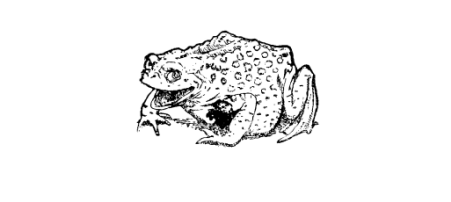
\includegraphics[scale=.5]{Toad}
  \end{center}



\SPELL[
  Name=Fool's Fire,
  Link=wizardry-fools-fire,
  Paradigm=Entropy,
  Save=Y (negate),
  Duration=Concentration,
  Counter=\mylink{Enervate}{wizardry-enervate} ,
  Keywords=Splittable,
  Target=Close or Nearby point
]



You project \DICE will-o'the-wisps into an area Close or Nearby.  The wisps
can move one range (Close to Nearby, Nearby to Far Away, etc) each Moment
for as long as you concentrate.  You can split the wisps up any way you like
but they can't be more than Far-Away from you.  The wisps do not shed heat,
do not require air, and can't be doused by water.  They shed a steady yellow
light the brightness of a torch.  At the top of the Moment, you can command
up to \DICE wisps to Befuddle up to \DICE Monsters.  The Monsters
immediately get a Save to negate (one for each wisp that's targetting them),
but a successful Save does not end the spell.  If any of the wisps are
struck by an Enervate spell, they are all dispelled if a Wizards' Duel is
lost.



\SPELL[
  Name=Greaseball,
  Link=wizardry-greaseball,
  Paradigm=Entropy,
  Save=N,
  Duration=Markovian,
  Counter=\mylink{Pritchard's Gusty Belch}{wizardry-pritchards-gusty-belch} (acid) ,
  Keywords=None,
  Target=Close or Nearby Monster or Object
]



Toss a small ball of grease at a point on the ground Close or Nearby. If you
would prefer to throw the ball at a person or object, make a Fight \RO using
your \INT - if you miss, it dissapates.  If thrown at the ground, the
surface becomes slick with a thick oil; anyone attempting to move through
the area must \RO using \DEX+\MD with a -\DICE penalty or immediately fall
Prone.  It requires a successful \RO to get up again.  If you throw it at a
creature, the effect is as above, plus they can't hold anything without
dropping it.  If you throw it at an object, the object becomes impossible to
carry or hold until the grease is removed with a mild or strong acid. 
Pritchard's Gusty Belch (acid variety) will dispel the grease if a Wizards'
Duel is lost; the grease is also highly flammable.  





\SPELL[
  Name=Grimm's Electric Fingers,
  Link=wizardry-grimms-electric-fingers,
  Paradigm=Elements,
  Save=Y (half),
  Duration=0,
  Counter=None ,
  Keywords=None,
  Target=Close or Nearby Monster or Object
]



Forks of lightning erupt from your oustretched hands, striking a Close or
Nearby target for \SUMDICE damage (Save for half). You can cause the
lightning to "jump" up to \DICE-1 times to another creature or object Close
by, provided they are conductive (iron armor, metal ladders, etc).  Magic
swords aren't conductive.  You can "ping-pong" between two objects if you
desire. Creatures struck by this secondary lightning bolt take \DICE damage
(no Save). Objects struck by this secondary lightning bolt will become
momentarily electrified, and deal a shock that could cause someone to lose
their grip unless they \RO : \VIG + \FOC with a -\DICE penalty.



\SPELL[
  Name=Hammerspace Mule,
  Link=wizardry-hammerspace-mule,
  Paradigm=Force,
  Save=N,
  Duration=Session,
  Counter=\mylink{Illusion}{wizardry-illusion} ,
  Keywords=Hammerspace,
  Target=Close
]



You create a spectral mule out of pure Force energy. The mule carries two
magical saddlebags that can each hold \SUMDICE Significant Items whose
combined weight doesn't exceed \DICE x 200kg (a reminder that a person is 25
Significant Items, and small creatures are 15).  The mule walks at a briks
trot.  It will stop and turn at your verbal command, but you cannot make it
reverse or slow down. You can only give it the commands "go", "stop",
"left", and "right". If the mule takes any damage, it immediately disappears
and drops all the items on the ground.  The mule will obey your last command
until the spell's duration expires.  Hammerspace Mules think that Illusions
are real; if the Illusion would damage them in some way (a pit they would
fall into, a spear they would run into, etc) the Mule is dispelled (dropping
its items on the ground) if a Wizards' Duel is lost.





\SPELL[
  Name=Helping Hand,
  Link=wizardry-helping-hand,
  Paradigm=Biomancy,
  Save=N,
  Duration=Concentration,
  Counter=\mylink{Web}{wizardry-web} ,
  Keywords=None,
  Target=Self
]



You can detach your hand from its wrist (your choice as to which one).  The
hand floats at chest height and can hold anything you could normally hold. 
The hand can't use any weapons except for an Ego Weapon.  It can grab
shirts, press buttons, and shove people (but not too hard).  If anyone
attacks the hand, you have to roll your Guard as if they were attacking you. 
If your hand takes any damage, it disappears for the rest of the Session. 
Additionally, if the Hand is ever caught in a Web spell, it will disappear
if a Wizards' Duel is lost.  At the end of the Session, roll a d6.  On a 1
or 2, the hand returns as normal next Session - otherwise, it comes back as
something else (a claw, a tentacle, etc) at the Arbiter's discretion.



\SPELL[
  Name=Heroic Leap,
  Link=wizardry-heroic-leap,
  Paradigm=Biomancy,
  Save=N,
  Duration=0,
  Counter=None ,
  Keywords=None,
  Target=Self or Close Ally
]



You and up to \DICE-1 allies can leap \VIG+\SUMDICE meters high and/or
\VIG+\SUMDICE meters forward in a straight line.  You take no damage on
landing, provided you land on or above the level you started from. For
example, you could leap from the ground to top of a steeple, or you could
leap over the steeple to land on the ground, but you couldn't leap from the
top of a steeple to the ground.  When you land, you can make a \RS : \DEX
(\RS : \INT if you are the caster) and if you succeed,
you can leap again. You can do this up to \DICE times.  You can't cast
spells or Fight while you're jumping around.





\SPELL[
  Name=Hollow Head,
  Link=wizardry-hollow-head,
  Paradigm=Biomancy,
  Save=N,
  Duration=Session,
  Counter=None ,
  Keywords=Hammerspace,
  Target=Self
]



You brain disappears and your head has a hinge that opens like a box, but
only you know this and only you can open it. For the rest of the Session,
you are immune to the next \DICE spells from the Mind paradigm, and you can
fit up to \SUMDICE Significant Items inside of your head in Hammerspace
(pulling one of these items out takes a Maneuver).  When you resist the
final Mind paradigm spell, the enchantment immediately ends. If the spell
ends while items are stored in your head they will mix with your
brain-matter. Usually this is fatal, though ambitious sorcerers sometimes
add drugs.  While your head is hollow, another sorcerer could read the
spell(s) inscribed on the inside.


  \begin{center}
  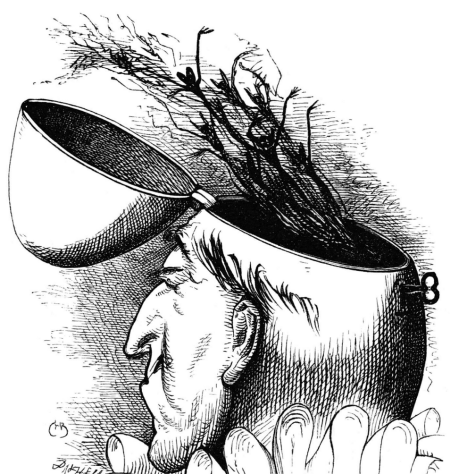
\includegraphics[scale=.5]{HollowHead}
  \end{center}





\SPELL[
  Name=Ice Bridge Step,
  Link=wizardry-ice-bridge-step,
  Paradigm=Elements,
  Save=N,
  Duration=Session,
  Counter=\mylink{Greaseball}{wizardry-greaseball} ,
  Keywords=None,
  Target=Self
]



You and up to \DICE-1 allies can run over liquids as if they were land.  Ice
forms beneath your feet with each step. If you slow down (to walk, fight,
etc), you'll sink. Very wavy seas may require you to \RS : \DEX.  Very hot
liquids (like lava) may require you to \RS : \INT.  The ability is dispelled
if you are struck by a Greaseball spell and you fail a Wizards' Duel.





\SPELL[
  Name=Icebolt,
  Link=wizardry-icebolt,
  Paradigm=Elements,
  Save=Y (half),
  Duration=0 / Markovian,
  Counter=None ,
  Keywords=None,
  Target=Close or Nearby point (straight line)
]



Throw a bolt of ice at a target Close or Nearby.  The bolt will travel in a
straight line from your fingers.  Anything touched by the bolt takes
\SUMDICE damage, Save for half.  Additionally, everything that fails its
Save is frozen to whatever surfaces they are touching.Keys are frozen in
their locks; swords are frozen to hands; boots are frozen to the ground
(creatures are usually immobilized from the boots down unless they were
playing in a fountain or something).  The objects are stuck until the
duration expires.  




\SPELL[
  Name=Illusion,
  Link=wizardry-illusion,
  Paradigm=Mind,
  Save=N,
  Duration=Varies,
  Counter=\mylink{Ego Weapon}{wizardry-ego-weapon} ,
  Keywords=None,
  Target=Varies
]



You create an illusion of anything you desire. If anything touches the
illusion, it will pass through it with no effect.  The illusion cannot be
greater than \DICE x \DICE meters in size.  Think of the illusion as a
perfectly accurate hologram that you are creating - the illusion can be
heard in addition to being seen, can perform the same action over and over
again, and can deliver messages, but it can't interact in a meaningful way
or perform complex actions based on external forces. 

Each aspect of the illusion requires one or more Blood die to cast:

\mylist {
  \item You want the illusion to say up to \DICE + \DICE words or make \DICE
+ \DICE sounds (wailing, shouting, etc)
  \item You want the illusion to be a physical thing (hole in the ground,
stone wall, orc guard, etc)
  \item You want the illusion to be able to move up to \DICE meters
  \item You want to cast the illusion on a living creature (disguise them as
a beggar or a lamp post)
}

Note that there is some Arbiter's discretion here.  A guard pacing in front
of a door might cost 2 \DICE (a physical thing moving back and forth 2
meters), but if you want the illusion of acrobats or pouncing lions it will
be more costly.  A disguise cast on someone to appear to be a beggar might
cost 1 [die] (a living creature wearing the face and clothing of a random
beggar), but disguising yourself as the king will be significantly harder.

The Illusion will last for \DICE Hours.  Anyone touching the illusion will
immediately know it to be fake, but this doesn't cause the illusion to
disappear.  However, if the illusion is touched with an Ego Weapon, it will
disappear if a Wizards' Duel is lost.





\SPELL[
  Name=Invisibility,
  Link=wizardry-invisibility,
  Paradigm=Entropy,
  Save=N,
  Duration=Varies,
  Counter=\mylink{Fool's Fire}{wizardry-fools-fire} ,
  Keywords=None,
  Target=Self or Close Allies or Objects
]



Up to \DICE objects or creatures can be made invisible (including yourself),
and will remain that way as long as they don't move.  As soon as the
creature or object moves (or is moved), the charm is broken.  Invisible
creatures can see other invisible and hidden objects (including Skulking
Knaves).  If this spell is cast on something Invisible, it will force the
object to become seen.  The duration of the charm depends on the dice
invested.  1 [die]: \SUMDICE Moments; 2 \DICE: Minutes; 3 \DICE: Hours; 4
\DICE Days; 5 \DICE: Weeks; 6+ \DICE: Forever.  The wisps from a Fool's Fire
can dispel the Invisibility of a Wizards' Duel is lost.

  \begin{center}
  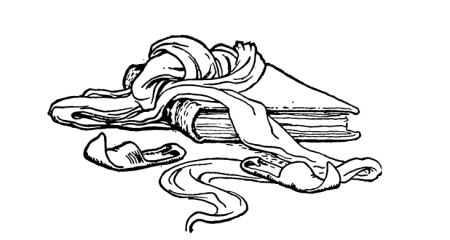
\includegraphics[scale=.5]{Invisibility}
  \end{center}





\SPELL[
  Name=Kelsier's Swarm of Irritating Vermin,
  Link=wizardry-kelsiers-swarm-of-irritating-vermin,
  Paradigm=Force,
  Save=N,
  Duration=Markovian,
  Counter=\mylink{Mighty Lungs}{wizardry-mighty-lungs} ,
  Keywords=None,
  Target=Close; Nearby; Far Away
]



You summon a cloud of tiny, magical, irritating vermin to an area Close,
Nearby, or Far-Away.  The vermin deal \DICE damage per Moment to every
living creature Close to them, but no damage to nonliving creatures or
objects. At the top of each Moment they are in the cloud, a non-mindless
creature must Save or take a -\DICE penalty on their Fight roll.  The vermin
won't move from the spot where they are summoned, and will remain until the
spell expires.  If the target is an object, the vermin will do minor
cosmetic damage, such as chewing holes in paper, gnawing wood, chipping
paint, and scratching glass.  Mighty Lungs will dispel the swarm if a
Wizards' Duel is lost.



\SPELL[
  Name=Knife Trick,
  Link=wizardry-knife-trick,
  Paradigm=Force,
  Save=N,
  Duration=Session,
  Counter=\mylink{Grimm's Electric Fingers}{wizardry-grimms-electric-fingers} ,
  Keywords=Splittable,
  Target=Close; Nearby; Far Away
]



Up to \DICE daggers orbit your head like a halo or crown.  These must be
daggers in your possession.  Magic and silver daggers are OK, as are other
"dagger-like" items (icicles, shards of glass, etc) at the Arbiter's
discretion.  At any time during the Session, you can mentally "throw" one or
more of these daggers at things that are Close, Nearby, or Far-Away with
unerring accuracy.  This could be used to sever a rope or pin something to a
wall (or stick into someone's chest) - but no Gambits, that wouldn't be
fair.  Each dagger does \SUMDICE+\DICE damage i.e. if you were to throw 1
dagger at someone, it would do d6+1, two daggers 2d6+2, etc.  Grimm's
Electric Fingers will dispel the magic and cause the daggers to fall to the
ground if a Wizards' Duel is lost.





\SPELL[
  Name=Knock,
  Link=wizardry-knock,
  Paradigm=Entropy,
  Save=N,
  Duration=0,
  Counter=\mylink{Lock}{wizardry-lock} ,
  Keywords=None,
  Target=Close or Nearby Objects
]



\DICE Close or Nearby object(s) is/are opened. Doors are flung wide, locks
are broken, shackles are bent open, belts come undone.  Ideas or thoughts
can be unlocked from a mind if a \RB : \INT contest is lost. Objects locked
by the Lock spell are opened if a Wizards' Duel is won.




\SPELL[
  Name=Levitating Disc,
  Link=wizardry-levitating-disc,
  Paradigm=Force,
  Save=N,
  Duration=Concentration,
  Counter=\mylink{Suspend Objects}{wizardry-suspend-objects} ,
  Keywords=None,
  Target=Close or Nearby point in space
]



You draw a circle \DICE meters in radius in the air. The inside of the
circle is made of Force, as solid as iron. You can cause the circle to
raise, lower, or hover in place.  You can only move up and down (never
side-to-side).  Up to \DICE people could stand under it and be completely
covered, or on it and be moved provided they don't weigh more than \DICE
x200kg.  If you lower the circle on top of someone, they take \DICE damage
per Moment. The circle moves 10 meters a minute (about 3m per Moment).  You
can draw the circle in any orientation, and you can change its orientation
at any time.  If the Levitating Disc is targeted with Suspend Objects, the
disc will be dispelled if a Wizards' Duel is lost.





\SPELL[
  Name=Lipby Chonk's Viscous Form,
  Link=wizardry-lipby-chonks-viscous-form,
  Paradigm=Biomancy,
  Save=N,
  Duration=Combat or \SUMDICE Minutes,
  Counter=None ,
  Keywords=None,
  Target=Self
]



Your flesh becomes gelatinous. You can squeeze through gaps as small as
keyhole with a great deal of effort. You take no damage from Crushing
attacks for the duration of the spell. The spell only affects your flesh,
not anything you're wearing or carrying.




\SPELL[
  Name=Lock,
  Link=wizardry-lock,
  Paradigm=Mind,
  Save=Y (negate),
  Duration=Markovian,
  Counter=None ,
  Keywords=None,
  Target=Close and Nearby Objects
]



Up to \DICE non-living thing slam shut and can't be opened. If the object is
a door, chest, or something like it, it will slam shut forcefully and
loudly. This spell can work on things that aren't portals (a sword could be
locked in its scabbard). You can also use this spell to lock a specific
memory or thought, making it immune to mind reading or scrying without a \RB
: \INT contest.  The duration is Markovian and depends on the number of
\DICE invested.  The Lock can be dispelled by the Knock spell if a Wizards'
Duel is lost.


\SPELL[
  Name=Meat Shield,
  Link=wizardry-meat-shield,
  Paradigm=Biomancy,
  Save=N,
  Duration=Combat or \SUMDICE Minutes ,
  Counter=None ,
  Keywords=None,
  Target=Close and Nearby
]

You summon a giant slab of meat.  The meat has \SUMDICE+\DICE Health, and
can fill an area \DICE meters cubed.  The meat weighs \DICE x100kg and lasts
for \DICE Hours.  Zoological creatures will attack the Meat Shield first. 
Up to \DICE other creatures can eat the Meat Shield in lieu of rolling their
Provisions, but the provenance of the meat is ... unknown.  If a Scything
Disc of Nog is used on a Meat Shield, the shield will be dispelled if a
Wizards' Duel is lost (otherwise, it will take damage as normal).





\SPELL[
  Name=Mighty Lungs,
  Link=wizardry-mighty-lungs,
  Paradigm=Biomancy,
  Save=N,
  Duration=Until exhalation,
  Counter=None ,
  Keywords=Contested,
  Target=Self
]

Your next inhalation allows you inhale 10x the normal amount of air. Not
only does this allow you to hold your breath for 10x as long, but if you
exhale forcefully it will release a blast of air strong enough to knock
pigeons out of air and polish your teeth. A human-sized creature is knocked
Prone and pushed Nearby unless they make a Contested roll using \DEX or \VIG
(their choice) with a -\DICE penalty.  This spell will also blow open all
the closed but unlocked doors in a room, shatter all the windows in a
building, or knock the thatched roof off a peasant's shack. If you cast this
spell with 3 or more \DICE, Save or your teeth shatter.




\SPELL[
  Name=Mirror Image,
  Link=wizardry-mirror-image,
  Paradigm=Entropy,
  Save=N,
  Duration=Combat or \SUMDICE Minutes,
  Counter=None ,
  Keywords=None,
  Target=Self
]



You create \DICE illusory images of yourself, which move as you move and
always stay Close to you. They are constantly stepping through each other,
so that it is impossible to tell which is which. When an enemy attacks you,
they'll always hit an image first.  An image vanishes as soon as it suffers
a solid impact (a blow from a mace, but also a slap). Area effects such as a
dragon's breath will cause all images to instantly vanish (and you take the
damage, naturally).





\SPELL[
  Name=Morass,
  Link=wizardry-morass,
  Paradigm=Elements,
  Save=N,
  Duration=Concentration,
  Counter=\mylink{Bastogne's Glamping Charm}{wizardry-bastognes-glamping-charm} ,
  Keywords=Contested,
  Target=Nearby or Far-Away Area
]



The ground \SUMDICE meters in radius and \DICE meters deep turns to black
muck.  Monsters and objects in the mud sink 1 meter a Moment.  At the top of
the Moment, a creature can make a Contested roll using \VIG with a -\DICE
penalty to pull themselves out 1 meter (if they were only 1 meter deep to
begin with, they escape).  If someone's head dips below the mud (2m for
people, 1m for Pooka, 4m or more for giants), they are immediately placed on
Death's Door, and have to roll their Death Die every turn they are under the
mud (they can still claw their way up 1m with a successful Contested roll,
as above).  If they don't have a Death Die, they die in \HD Moments.

The spell lasts for as long as you concentrate.  When you break your
concentration, everything that sunk in the mud is immediately thrown back to
the surface.   If the area covered by the Morass is targeted by Bastogne's
Glamping Charm, the Morass will be dispelled (and the objects brought to the
surface) if a Wizards' Duel is lost.




\SPELL[
  Name=Negasonic Bomb,
  Link=wizardry-negasonic-bomb,
  Paradigm=Mind,
  Save=N,
  Duration=Concentration,
  Counter=\mylink{Cacaphony}{wizardry-cacaphony} ,
  Keywords=None,
  Target=Nearby or Far Away Area
]



You roll a small orb of Mind to a point Close, Nearby or Far-Away; the orb
rolls silently and is hard to see.  When the orb stops rolling it
immediately and silently detonates.  Creatures Close to the designated point
are Deafened until they leave the area of effect.  Likewise, no spells can
be cast while Close to the Negasonic Bomb.  Skulking effects (including
Murder) succeed automatically while in range.  The spell lasts as long as
you concentrate.  The bomb can be dispelled by Cacaphony if a Wizards' Duel
is lost.





\SPELL[
  Name=Prismatic Ray,
  Link=wizardry-prismatic-ray,
  Paradigm=Entropy,
  Save=Y (half),
  Duration=0,
  Counter=None ,
  Keywords=Splittable,
  Target=Nearby or Far-Away
]



A brilliant white light emanates from your forehead to a point Nearby or
Far-Away, where it splits into a prism of \DICE beams.  Each beam strikes a
random Ally or Monster Close to the prism.  Roll a d8 on the table below for
each beam and apply its results.

\mynumlist {
  \item \mybold{Red} Target takes \DICE fire damage, Save for half. Highly flammable things catch fire.
  \item \mybold{Orange}  Target takes \DICE bashing damage, Save for half. 
  \item \mybold{Yellow} Target takes \DICE lightning damage, Save for half.  If you fail your Save, you drop what you're holding.
  \item \mybold{Green} Target takes \DICE acid damage, Save for half. Roll your Armor \UD if applicable.
  \item \mybold{Blue} Target takes \DICE ice damage, Save for half. If you fail your Save, you fall Prone.
  \item \mybold{Indigo} Target takes \DICE stabbing damage, Save for half.
  \item \mybold{Violet} Target takes \DICE chopping damage, Save for half.
  \item \mybold{Roll} again.  Instead of \DICE damage, the effect deals \SUMDICE damage.. If you get this result again, the beam splits and the target takes an additional effect (roll again and apply the result).  Continue in this wayuntil you don't roll an 8.
}





\SPELL[
  Name=Pritchard's Gusty Belch,
  Link=wizardry-pritchards-gusty-belch,
  Paradigm=Biomancy,
  Save=N,
  Duration=0,
  Counter=None ,
  Keywords=None,
  Target=Close and Nearby Area
]



You can breathe up to \DICE elements (fire, acid, water, wind, steam, etc)
immediately in front of you for a Moment.  The elements don't interact with
one another and act independently, so if you were to belch out fire and
water, you would get the effects of both.  If the order matters (set
something on fire and immediately douse it with water), you pick the order
of effects.  Water breath is enough to extinguish fires smaller than a big
bonfire, or wash off acid; wind breath could push a small sailboat or blow
swarming insects out of an area; acid breath bleaches the color from objects
and irritates the eyes; fire breath would cause paper and flammable objects
(but not people, unless they were doused in oil) to catch fire, etc.




\SPELL[
  Name=Protection from Element,
  Link=wizardry-protection-from-element,
  Paradigm=Elements,
  Save=N,
  Duration=Session,
  Counter=\mylink{Prismatic Ray}{wizardry-prismatic-ray} ,
  Keywords=None,
  Target=Self or Close Ally
]



Reduce all damage of a single chosen element (acid, cold, fire, lightning,
etc) by -\DICE.  The spell protects its targets from the negative effects of
the natural elements (desert heat, arctic chill) as well.  If you are struck
by a Prismatic Ray of the same elemental type, the protection is dispelled
if a Wizards' Duel is lost.


  \begin{center}
  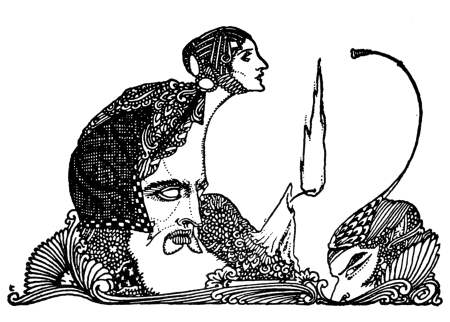
\includegraphics[scale=.5]{Wizardry_1}
  \end{center}



\SPELL[
  Name=Rhea's Efficacious Plow,
  Link=wizardry-rheas-efficacious-plow,
  Paradigm=Force,
  Save=N,
  Duration=Moments,
  Counter=None ,
  Keywords=None,
  Target=See description
]



You send an invisible wedge of Force along the ground in a straight line up
to a Distant point.  The wedge can take up to \DICE turns ("left" or
"right") at your command.  Any light debris on the path (snow, small stones,
leaves, grass) is pushed to the side; fields can be tilled. Any pressure
plates or tripwires are activated. You do not have to be able to see the
entire path, but you do need to know the approximate route the wedge will
take. The wedge can't move through solid objects, and it can't hurt anyone.
The path cleared is \DICE meters wide. If you cast this spell with 3 \DICE
or more, the width becomes \SUMDICE meters wide.




\SPELL[
  Name=Sandstorm,
  Link=wizardry-sandstorm,
  Paradigm=Elements,
  Save=N,
  Duration=Concentration,
  Counter=None ,
  Keywords=None,
  Target=Close
]



You cough up a swirling spiral of sand.  Small flying creatures (bug-sized),
arrows, and spears cannot enter or leave the sandstorm.  Up to \DICE-1 other
people can hide in the sandstorm with you.  The sand moves with you and
lasts as long as you concentrate.



\SPELL[
  Name=Sanguine Mail,
  Link=wizardry-sanguine-mail,
  Paradigm=Biomancy,
  Save=N,
  Duration=Session,
  Counter=\mylink{Enervate}{wizardry-enervate} ,
  Keywords=None,
  Target=Self
]



You become encased in elaborate plate mail that seems to be made from
constantly congealing blood.  You definitely stand out in a crowd. Your \MD
drops to d4, but you can still cast spells.  The \UD for the Armor depends
on the number of \DICE invested: 1 d3; 2 d4; 3 d6; 4 d8; 5 d10; 6+ d12.  If
you are struck with an Enervate spell, the Sanguine Mail is dispelled if a
Wizards' Duel is lost.





\SPELL[
  Name=Scuttle,
  Link=wizardry-scuttle,
  Paradigm=Biomancy,
  Save=N,
  Duration=Combat or \SUMDICE Minutes,
  Counter=\mylink{Greaseball}{wizardry-greaseball} ,
  Keywords=None,
  Target=Self
]



Your clothes and hair animate to carry you around. You can move at full
speed in any orientation, and you can freely rotate as you move. For
instance, you could run while standing on your head, holding a torch, and
turning counterclockwise. You can lie on your side and, while flipping end
over end, move backwards. This effect does not allow you to climb up walls,
but ladders and ropes are no problem (you could suspend yourself from a rope
and cast spells, for example).  If you are struck with a Greaseball, or
attempt to climb something affected by Greaseball, the Scuttle is dispelled
if a Wizards' Duel is lost.




\SPELL[
  Name=Scything Disc of Nog,
  Link=wizardry-scything-disc-of-nog,
  Paradigm=Force,
  Save=Y (half),
  Duration=0,
  Counter=None ,
  Keywords=None,
  Target=Nearby or Far Away Area
]



You hurl a whirling disc of Force and light from your fingertip. The disc
screeches like a sawblade. It deals \SUMDICE damage to its target, Save for
half. If it deals more than 6 damage, it bounces towards a random creature
(friend, foe, or even yourself) Close or Nearby, dealing \SUMDICE-2
damage, Save for half. If it deals more than 6 damage, it bounces towards
another random creature Close or Nearby, dealing \SUMDICE-4 damage, Save for
half. This continues, losing 2 damage with each bounce, until there are no
valid targets or the spell deals 6 or less damage to a creature.





\SPELL[
  Name=Sleep,
  Link=wizardry-sleep,
  Paradigm=Mind,
  Save=Y (negate),
  Duration=Markovian,
  Counter=\mylink{Cacaphony}{wizardry-cacaphony} ,
  Keywords=None,
  Target=Close or Nearby Area
]



You summon a cloud of somnomulent dust to a point Close or Nearby. 
\SUMDICE creatures Close to the cloud, who have no more than \DICE \HD, must
immediately Save or fall into a magical slumber.   They can't be awakened by
anything less than a vigorous slap (counts as a Maneuver).  You don't have
control over who falls asleep, it's entirely random and will be as many
creatures as possible (up to \SUMDICE).  You are immune to your own Sleep
spell (so you could cast it Close to yourself).  Creatures who fall asleep
immediately fall Prone and drop any items they're holding.  Fight rolls
agains them will hit automatically and do maximum damage, and can only be
blocked by Armor.  This will wake the creature up, of course.  If an orb of
Cacaphony is detonated Nearby, the creatures will awaken if a Wizards' Duel
is lost.  Otherwise, creatures who fall asleep will remain asleep for the
Markovian duration.   




\SPELL[
  Name=Summon Candles,
  Link=wizardry-summon-candles,
  Paradigm=Force,
  Save=N,
  Duration=Varies,
  Counter=\mylink{Fogbank}{wizardry-fogbank} ,
  Keywords=None,
  Target=Close
]



\SUMDICE dribbling candles appear on objects you touch. You can walk around
placing candles as required for Minutes. The candles are lit and burn for
Hours. They can be detached, but will fade from existence within Minutes. 
For every 6 candles placed Close to one another, the wizard close to the
candles gains 1 of the following (your choice): Safe Casting: Replace one of
your rolled Blood Die with a natural 1; Power Casting: Replace one of your
rolled Blood Die with a natural 6; Natural Casting: add a natural +1 to any
Blood Die you've rolled.  When you use 1 of these powers, the 6
candles immediately disappear.  Note that \myital{any} sorcerer can use these
abilities, friend or foe.  A philosopher will immediately know if they are in
an area of candles, and what powers it can bestow on them.  If the candles
are encased in a Fogbank, they are snuffed out and dispelled if a Wizards'
Duel is lost.





\SPELL[
  Name=Suspend Objects,
  Link=wizardry-suspend-objects,
  Paradigm=Force,
  Save=Y (negate),
  Duration=Concentration,
  Counter=\mylink{Levitating Disc}{wizardry-levitating-disc} ,
  Keywords=None,
  Target=Any Distance
]



You can hold up to \DICE objects in the air, weighing no more than \DICE
x200kg.  You can allow these objects to descend at 3m per Moment at your
discretion. Creatures who are brought to ground in this way take no falling
damage.  Unwilling creatures (flying Monsters, for example) get a Save to
negate.  If a Levitating Disc is summoned in the midst of the held
creatures, the Suspend Objects spell will be dispelled (and the objects will
fall) if a Wizards' Duel is lost.




\SPELL[
  Name=Tempestuous Chariot,
  Link=wizardry-tempestuous-chariot,
  Paradigm=Elements,
  Save=N,
  Duration=One trip,
  Counter=None ,
  Keywords=None,
  Target=Close
]



A tumult of air elementals lifts you and \DICE-1 others and takes you in any
direction the you desire, up to \SUMDICE km away.   One catch - the
elementals can only travel in a straight line, and you have to choose
beforehand the way to go ("up", "east", "that way", etc).  While you are in
the tempest you are buffeted horribly and can neither talk nor act.  The
winds refuse to travel without you, and will immediately dispel if you lose
contact




\SPELL[
  Name=Vertigo,
  Link=wizardry-vertigo,
  Paradigm=Mind,
  Save=Y (negate),
  Duration=Markovian,
  Counter=\mylink{Suspend Objects}{wizardry-suspend-objects} ,
  Keywords=None,
  Target= Any Distance
]



You can cause up to \DICE Close, Nearby, Far-Away, or Distant creatures to
suffer severe vertigo unless they Save.  Creatures that are climbing or
flying immediately fall; creatures who are Close to the edge of something (a
cliff, a wall, the guardrails of a ship, etc) need to \RS : \FOC or fall.
Creatures already on the ground will fall Prone.  If the creatures are
struck with a Suspend Objects spell, the Vertigo is dispelled if a Wizards'
Duel is lost.




  \begin{center}
  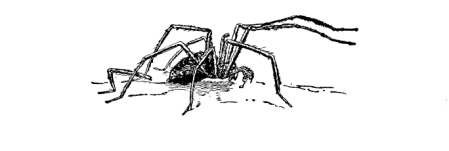
\includegraphics[scale=.5]{Spider}
  \end{center}


\SPELL[
  Name=Web,
  Link=wizardry-web,
  Paradigm=Entropy,
  Save=Y (negate),
  Duration=Markovian,
  Counter=None ,
  Keywords=None,
  Target=Nearby or Far Away Area
]



You can anchor a giant web between three or more solid points up to \DICE
meters in radius (for example: the 4 points of a door, two trees and the
ground, across a hallway, etc).  Objects that touch the web immediately
become stuck; arrows and spears can't be fired through it.  Creatures that
enter the web (or are caught in it when cast) must Save or become ensnared
for the Markovian duration (each creature should roll their Markovian die
separately). Fight rolls against them hit automatically and can only be
blocked by Armor.  The web is extremely flammable and will be consumed in
\DICE Moments.



\SPELL[
  Name=Whirling Blades,
  Link=wizardry-whirling-blades,
  Paradigm=Entropy,
  Save=N,
  Duration=Concentration,
  Counter=\mylink{Suspend Objects}{wizardry-suspend-objects} ,
  Keywords=None,
  Target=Self
]



You summon a number of invisible blades of Force that spin around your
waist, with you in the center.  Every creature Close to you takes \DICE
damage for each Moment the spell is maintained.  The blades will cut or
damage fragile objects.  If the creature or object sits above or below your
waist, they take no effect.  If the blades are struck by a Suspend Objects
spell, they will be dispelled if a Wizards' Duel is lost.





  
}%end

